%************************************************
\chapter[Appendix 3.1: Chapter 3 - Model parameterization]{Appendix 3.1: Chapter 3 - Model parameterization and implementation}\label{ch:Appendix3.1}
%************************************************
\renewcommand{\thefigure}{A.3.1.\arabic{figure}}
\setcounter{figure}{0}

\renewcommand{\thetable}{A.3.1.\arabic{table}}
\setcounter{table}{0}

\section*{Model parameterization}\label{model-parameterization}

The parameters of the model from Chapter 3 refer to properties of 1) the whole community, 2) the strength of each interaction type, or 3) species performance. In the tables, the following abbreviations are used: AM = amensalism, AN = antagonism, CM = commensalism, CP = competition, M = mutualism.

\begin{longtable}[]{@{}ll@{}}
\caption[Model community parameters]{\color{Gray}Community-level parameters.}
\label{tab:tableApp3.1.1}\\
\toprule
\begin{minipage}[t]{0.39\columnwidth}\raggedright\strut
Initial number of species\strut
\end{minipage} & \begin{minipage}[t]{0.55\columnwidth}\raggedright\strut
\{20, 40, 60\}\strut
\end{minipage}\tabularnewline
\begin{minipage}[t]{0.39\columnwidth}\raggedright\strut
Initial Interaction Type Ratio\strut
\end{minipage} & \begin{minipage}[t]{0.55\columnwidth}\raggedright\strut
\{\{AM = 0.2, AN = 0.2, CM = 0.2, CP = 0.2, M = 0.2\}, \{AM = 0.4, AN =
0.15, CM = 0.15, CP = O.15, M = 0.15\}, \{AM = 0.15, AN = 0.4, CM =
0.15, CP = O.15, M = 0.15\}, \{AM = 0.15, AN = 0.15, CM = 0.4, CP =
O.15, M = 0.15\}, \{AM = 0.15, AN = 0.15, CM = 0.15, CP = O.4, M =
0.15\}, \{AM = 0.15, AN = 0.15, CM = 0.15, CP = O.15, M = 0.4\}\}\strut
\end{minipage}\tabularnewline
\begin{minipage}[t]{0.39\columnwidth}\raggedright\strut
Overall connectance\strut
\end{minipage} & \begin{minipage}[t]{0.55\columnwidth}\raggedright\strut
0.5\strut
\end{minipage}\tabularnewline
\begin{minipage}[t]{0.39\columnwidth}\raggedright\strut
Initial SAD\strut
\end{minipage} & \begin{minipage}[t]{0.55\columnwidth}\raggedright\strut
Gambin\strut
\end{minipage}\tabularnewline
\begin{minipage}[t]{0.39\columnwidth}\raggedright\strut
Initial SAD parameters\strut
\end{minipage} & \begin{minipage}[t]{0.55\columnwidth}\raggedright\strut
\(\alpha\) = 2\strut
\end{minipage}\tabularnewline
\begin{minipage}[t]{0.39\columnwidth}\raggedright\strut
Number of discrete trophic levels\strut
\end{minipage} & \begin{minipage}[t]{0.55\columnwidth}\raggedright\strut
4\strut
\end{minipage}\tabularnewline
\begin{minipage}[t]{0.39\columnwidth}\raggedright\strut
Trophic level abundance scaling exponent\strut
\end{minipage} & \begin{minipage}[t]{0.55\columnwidth}\raggedright\strut
0.75\strut
\end{minipage}\tabularnewline
\begin{minipage}[t]{0.39\columnwidth}\raggedright\strut
Abundance of basal trophic level\strut
\end{minipage} & \begin{minipage}[t]{0.55\columnwidth}\raggedright\strut
100 \(*\) initial number of species\strut
\end{minipage}\tabularnewline
\bottomrule
\end{longtable}

\newpage

\begin{longtable}[]{@{}lll@{}}
\caption[Interaction probabilities]{\color{Gray}Probabilities of occurrence of each interaction type (\cref{fig:fig3.1} of chapter 3). The complete list of studies included can be found at the online supplementary material of the published article: https://esajournals.onlinelibrary.wiley.com/doi/abs/10.1002/ecy.2465}
\label{tab:tableApp3.1.2}\\
\toprule
Interaction & Trophic levels & Prob\tabularnewline
\midrule
\endhead
Amensalism & same & 1\tabularnewline
Amensalism & adjacent & 0\tabularnewline
Amensalism & other & 0\tabularnewline
Antagonism & same & 0.015\tabularnewline
Antagonism & adjacent & 0.918\tabularnewline
Antagonism & other & 0.067\tabularnewline
Commensalism & same & 0.661\tabularnewline
Commensalism & adjacent & 0.292\tabularnewline
Commensalism & other & 0.047\tabularnewline
Competition & same & 0.979\tabularnewline
Competition & adjacent & 0.021\tabularnewline
Competition & other & 0\tabularnewline
Mutualism & same & 0.048\tabularnewline
Mutualism & adjacent & 0.854\tabularnewline
Mutualism & other & 0.098\tabularnewline
\bottomrule
\end{longtable}

%\newpage

The range of $k$ parameters was chosen so that antagonistic interactions had a greater effect than other types, as they usually result in the death of the prey. In the same vein, the a parameter is an order of magnitude smaller for antagonistic interactions due to assumed defense mechanisms by resource species. The x\textsubscript{0} parameter does not have a specific ecological meaning in the context of our study, so we chose to keep it constant.

\begin{longtable}[]{@{}ll@{}}
\caption[Model interaction parameters]{\color{Gray}Interaction-level parameters.}
\label{tab:tableApp3.1.3}\\
\toprule
\begin{minipage}[t]{0.08\columnwidth}\raggedright\strut
k\strut
\end{minipage} & \begin{minipage}[t]{0.56\columnwidth}\raggedright\strut
\{AM = 0.1, AN = 0.5, CM = 0.1, CP = 0.1, M = 0.1\}\strut
\end{minipage}\tabularnewline
\begin{minipage}[t]{0.08\columnwidth}\raggedright\strut
a\strut
\end{minipage} & \begin{minipage}[t]{0.56\columnwidth}\raggedright\strut
\{AM = 0.01, AN = 0.001, CM = 0.01, CP = 0.01, M = 0.01\}\strut
\end{minipage}\tabularnewline
\begin{minipage}[t]{0.08\columnwidth}\raggedright\strut
x\textsubscript{0}\strut
\end{minipage} & \begin{minipage}[t]{0.56\columnwidth}\raggedright\strut
1\strut
\end{minipage}\tabularnewline
\bottomrule
\end{longtable}

\newpage

Basal species were assumed to have positive intrinsic growth rates, as opposed to species in higher trophic levels. Other parameters were in the range used by \cite{Garcia-Algarra2014}, the initial formulation of \cref{eq:eq3.5} in Chapter 3.

\begin{longtable}[]{@{}ll@{}}
\caption[Model species parameters]{\color{Gray}Species-level parameters.}
\label{tab:tableApp3.1.4}\\
\toprule
\begin{minipage}[t]{0.13\columnwidth}\raggedright\strut
r\strut
\end{minipage} & \begin{minipage}[t]{0.30\columnwidth}\raggedright\strut
basal species: (0,0.08) consumers: (-0.08,0)\strut
\end{minipage}\tabularnewline
\begin{minipage}[t]{0.13\columnwidth}\raggedright\strut
c\strut
\end{minipage} & \begin{minipage}[t]{0.30\columnwidth}\raggedright\strut
0.001\strut
\end{minipage}\tabularnewline
\begin{minipage}[t]{0.13\columnwidth}\raggedright\strut
\(\alpha\)\strut
\end{minipage} & \begin{minipage}[t]{0.30\columnwidth}\raggedright\strut
(1 \(*\) 10\textsuperscript{-5},1 \(*\) 10\textsuperscript{-4})\strut
\end{minipage}\tabularnewline
\bottomrule
\end{longtable}

\section*{Model implementation}\label{model-implementation}

The model is developed in R 3.0 \citep{RCoreTeam2018}, and makes use, mainly, of the package deSolve \citep{Soetaert2012} and the package suite tidyverse (www.tidyverse.org) for generation and treatment of results. Here we show how communities are assembled in terms of 1) their distribution of abundances and trophic levels, and 2) their interaction networks. In the last section, we expand on how model parameters are selected for solving the dynamical system.

\begin{figure}[ht]
\centering
\includegraphics[width=\textwidth]{./Figures/Appendix3_1/Fig_1.png}
\caption[Model diagram]{\color{Gray} Conceptual diagram of the model, showing 20 model species and two interaction types (solid and dashed lines). Abundances are proportional to the size of the node. The process depicted is replicated 1000 times for each configuration of species richness and frequency of interaction types.}
\label{fig:figApp3.1.1}
\end{figure}

\subsection*{Community assembly process}\label{community-assembly-process}

\subsubsection*{1. Abundance and trophic level structure}\label{abundance-and-trophic-level-structure}

The initial abundances of species and its (discrete) trophic level (first and second box of Fig. \ref{fig:figApp3.1.1}) are calculated by a function named \texttt{AssignTrophicLevel}. This function is able generate communities of any number of species and discrete trophic levels, with different initial SADs, and with or without abundance scaling with trophic level. We will show the workflow of this function by ``building'' a community with the following parameters, similar to the model communities analyzed in chapter 3:\\

\small

\begin{Shaded}
\begin{Highlighting}[]
\CommentTok{# number of species}
\NormalTok{num.sp <-}\StringTok{ }\DecValTok{40}
\CommentTok{# number of discrete trophic levels}
\NormalTok{trophic.levels <-}\StringTok{ }\DecValTok{4}
\CommentTok{# SAD parameters}
\NormalTok{abundance.distribution <-}\StringTok{ "gambin"}
\NormalTok{gambin.alpha <-}\StringTok{ }\DecValTok{2}
\NormalTok{gambin.maxoctave <-}\StringTok{ }\DecValTok{8}
\CommentTok{# include abundance scaling with trophic level}
\NormalTok{scaling.law.tl <-}\StringTok{ }\OtherTok{TRUE}
\CommentTok{# with exponent 3/4}
\NormalTok{scaling.exponent.tl <-}\StringTok{ }\FloatTok{0.75}
\CommentTok{# aggregated abundance of the basal trophic level, necessary for the scaling}
\NormalTok{basal.abundance <-}\StringTok{ }\NormalTok{num.sp *}\StringTok{ }\DecValTok{100}
\end{Highlighting}
\end{Shaded}

\normalsize
The first task is to calculate the aggregated abundances of each trophic level, according to the scaling. We added a small white noise term \(\epsilon \sim N(0,abundance/10)\) to introduce an element of small variability:\\

\small

\begin{Shaded}
\begin{Highlighting}[]
\NormalTok{trophic.level.abundance <-}\StringTok{ }\KeywordTok{numeric}\NormalTok{(trophic.levels)}
\NormalTok{trophic.level.abundance[}\DecValTok{1}\NormalTok{] <-}\StringTok{ }\NormalTok{basal.abundance}

\CommentTok{# calculate abundance for each trophic level}
\CommentTok{# including a white noise term with mean = 0 and sd = abundance/10}
\NormalTok{if(}\KeywordTok{length}\NormalTok{(trophic.level.abundance) >}\StringTok{ }\DecValTok{1}\NormalTok{)\{}
  \NormalTok{for(i.trophic.level in }\DecValTok{2}\NormalTok{:trophic.levels)\{}
    \NormalTok{trophic.level.abundance[i.trophic.level] <-}\StringTok{ }
\StringTok{      }\NormalTok{trophic.level.abundance[i.trophic.level -}\StringTok{ }\DecValTok{1}\NormalTok{]^scaling.exponent.tl }
    \NormalTok{trophic.level.abundance[i.trophic.level] <-}\StringTok{ }
\StringTok{      }\NormalTok{trophic.level.abundance[i.trophic.level] +}\StringTok{ }
\StringTok{      }\KeywordTok{rnorm}\NormalTok{(}\DataTypeTok{n =} \DecValTok{1}\NormalTok{,}\DataTypeTok{mean =} \DecValTok{0}\NormalTok{,}\DataTypeTok{sd =} \NormalTok{trophic.level.abundance[i.trophic.level]/}\DecValTok{10}\NormalTok{)}
  \NormalTok{\}}
\NormalTok{\}}
\end{Highlighting}
\end{Shaded}

\normalsize
This gives the following abundances (rounded to integer) for the four trophic levels defined:\\
\small

\begin{verbatim}
[1] 4000  489  112   34
\end{verbatim}

\normalsize

Next, the abundance of each species is drawn from the distribution specified, in this case, a discrete gambin with \(\alpha = 2\). We developed a function \texttt{GenerateProbNumbers} to incorporate this functionality in our model. Further details on how the function deals with the transformation from octaves to actual abundances can be checked in the documentation and code of the function.\\
\small

\begin{Shaded}
\begin{Highlighting}[]
\NormalTok{abundance.list <-}\StringTok{ }\NormalTok{DGC::}\KeywordTok{GenerateProbNumbers}\NormalTok{(}\DataTypeTok{times =} \NormalTok{num.sp,}
                                           \DataTypeTok{dist =} \NormalTok{abundance.distribution,}
                                           \DataTypeTok{cum.sum =} \KeywordTok{sum}\NormalTok{(trophic.level.abundance),}
                                           \DataTypeTok{gambin.alpha =} \NormalTok{gambin.alpha,}
                                           \DataTypeTok{gambin.maxoctave =} \NormalTok{gambin.maxoctave)}
\end{Highlighting}
\end{Shaded}

\normalsize
returns the following abundance distribution:\\

\begin{figure}[ht]
\centering
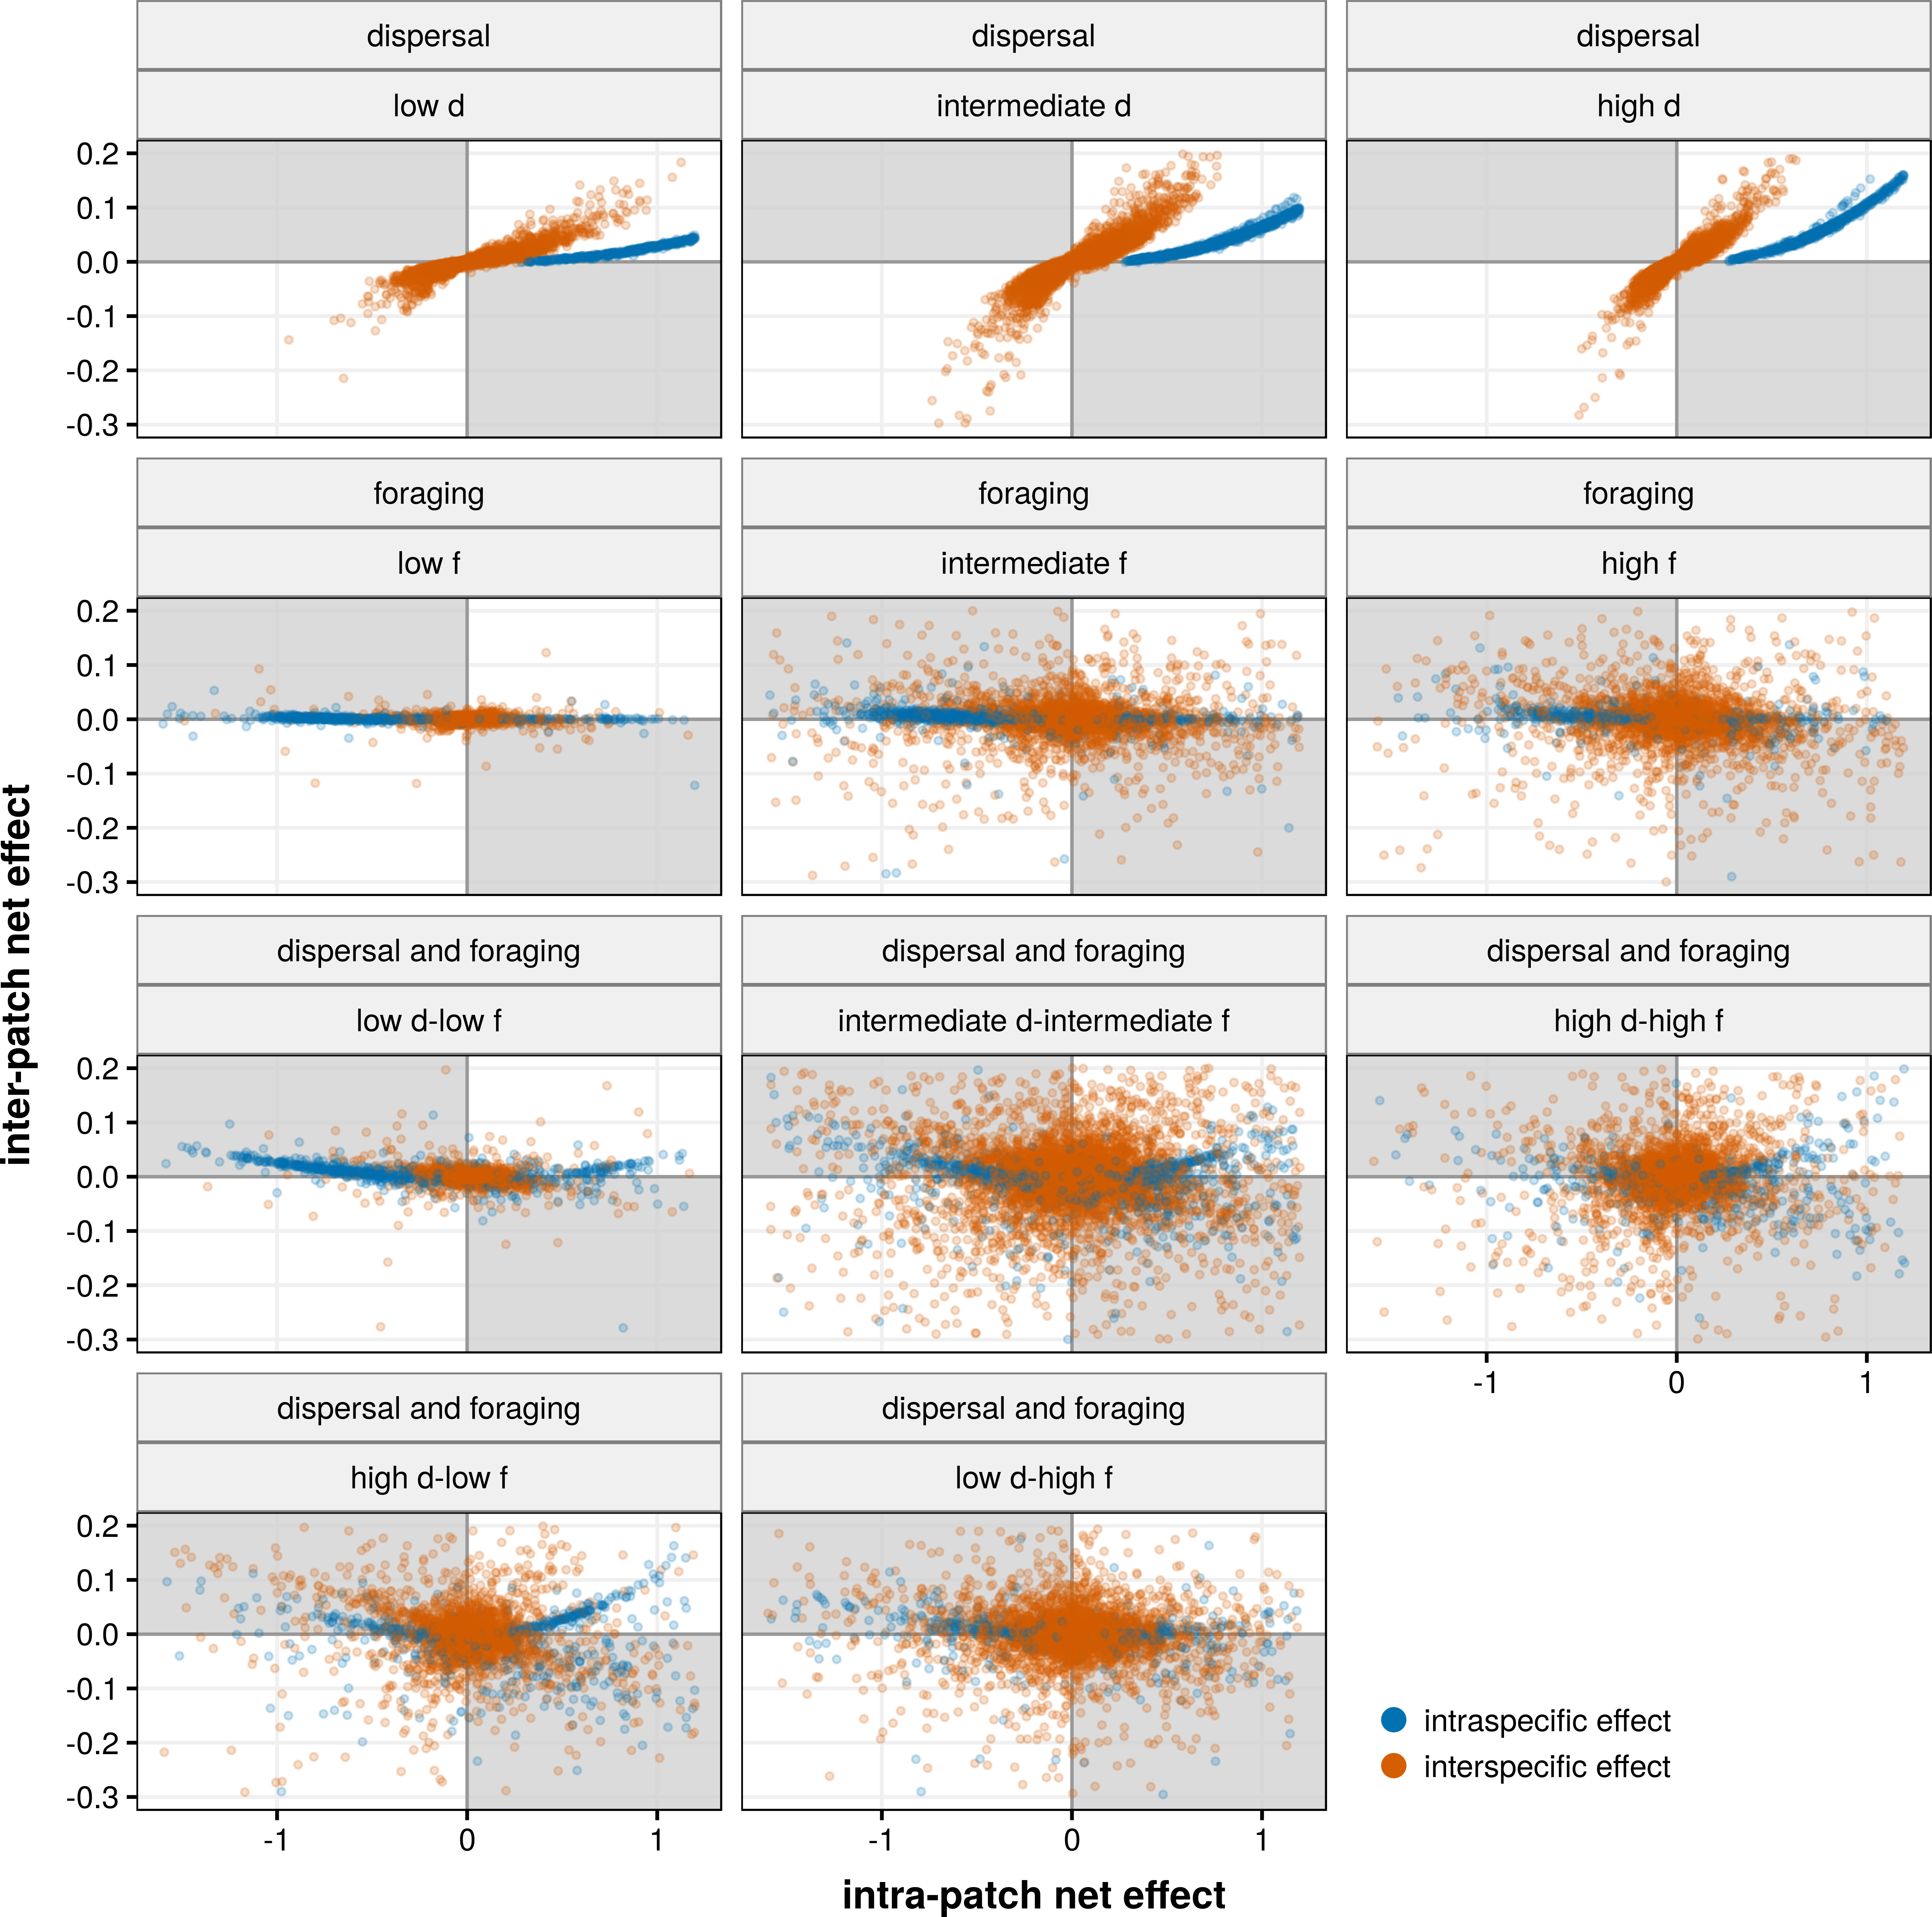
\includegraphics[width=\textwidth]{./Figures/Appendix3_1/Fig_2.png}
\caption[Abundance distribution]{\color{Gray} Abundance distribution for a community of 40 species generated with the parameterization of the main simulations.}
\label{fig:figApp3.1.2}
\end{figure}

At this stage, species have initial abundances but are not assigned to trophic levels. The next piece of R code assigns species to trophic levels ensuring that the aggregated abundances of a trophic level are consisten with the scaling already calculated. Again, a certain tolerance is allowed, so that abundances will not need to exactly follow the expected scaling.\\

\small

\begin{Shaded}
\begin{Highlighting}[]
\CommentTok{# create the dataframe}
\NormalTok{tl.results <-}\StringTok{ }\KeywordTok{data.frame}\NormalTok{(}\DataTypeTok{species =} \KeywordTok{c}\NormalTok{(}\DecValTok{1}\NormalTok{:}\KeywordTok{length}\NormalTok{(abundance.list)), }
                         \DataTypeTok{abundance =} \KeywordTok{sort}\NormalTok{(abundance.list,}\DataTypeTok{decreasing =} \NormalTok{T), }
                         \DataTypeTok{trophic.level =} \DecValTok{0}\NormalTok{)}

\CommentTok{# the most abundant species will always be at the basal level}
\NormalTok{tl.results\$trophic.level[}\DecValTok{1}\NormalTok{] <-}\StringTok{ }\DecValTok{1}

\NormalTok{for(i.tl in trophic.levels:}\DecValTok{1}\NormalTok{)\{}

  \CommentTok{# iterative process: add species until a trophic level is "filled".}
  \CommentTok{# For convenience I start in the upper trophic level, }
  \CommentTok{# since it will be the most difficult to fill }
  \CommentTok{# (few species will have such low abundances)}

  \NormalTok{if(i.tl ==}\StringTok{ }\DecValTok{1}\NormalTok{)\{}
    \NormalTok{my.abund <-}\StringTok{ }\NormalTok{tl.results\$abundance[}\DecValTok{1}\NormalTok{]}
  \NormalTok{\}else\{}
    \NormalTok{my.abund <-}\StringTok{ }\DecValTok{0}
  \NormalTok{\}}

  \CommentTok{# certain tolerance, it does not need to be exact}
  \NormalTok{tl.tolerance <-}\StringTok{ }\NormalTok{trophic.level.abundance[i.tl]*}\FloatTok{0.1}

  \NormalTok{my.sp <-}\StringTok{ }\DecValTok{0}

  \CommentTok{# while the abundance of the i.tl trophic level is not within the tolerance levels, }
  \CommentTok{# keep adding species}
  \NormalTok{while(}\KeywordTok{length}\NormalTok{(my.sp) !=}\StringTok{ }\DecValTok{0} \NormalTok{&}\StringTok{ }
\StringTok{        }\KeywordTok{findInterval}\NormalTok{(my.abund,}\KeywordTok{c}\NormalTok{(trophic.level.abundance[i.tl] -}\StringTok{ }\NormalTok{tl.tolerance,}
                                \NormalTok{trophic.level.abundance[i.tl] +}\StringTok{ }\NormalTok{tl.tolerance)) !=}\StringTok{ }\DecValTok{1}\NormalTok{)\{}

    \CommentTok{# potential species}
    \NormalTok{my.sp <-}\StringTok{ }\KeywordTok{which}\NormalTok{(tl.results\$trophic.level ==}\StringTok{ }\DecValTok{0} \NormalTok{&}\StringTok{ }
\StringTok{                     }\NormalTok{tl.results\$abundance +}\StringTok{ }\NormalTok{my.abund <}\StringTok{ }
\StringTok{                     }\NormalTok{(trophic.level.abundance[i.tl] +}\StringTok{ }\NormalTok{tl.tolerance))}

    \CommentTok{# sample from the potential species pool}
    \NormalTok{if(}\KeywordTok{length}\NormalTok{(my.sp)>}\DecValTok{0}\NormalTok{)\{}
      \NormalTok{my.sp <-}\StringTok{ }\KeywordTok{ifelse}\NormalTok{(}\KeywordTok{length}\NormalTok{(my.sp) ==}\StringTok{ }\DecValTok{1}\NormalTok{,my.sp,}\KeywordTok{sample}\NormalTok{(my.sp,}\DataTypeTok{size =} \DecValTok{1}\NormalTok{))}
      \NormalTok{my.abund <-}\StringTok{ }\NormalTok{my.abund +}\StringTok{ }\NormalTok{tl.results\$abundance[tl.results\$species ==}\StringTok{ }\NormalTok{my.sp]}
      \NormalTok{tl.results\$trophic.level[tl.results\$species ==}\StringTok{ }\NormalTok{my.sp] <-}\StringTok{ }\NormalTok{i.tl}
    \NormalTok{\}}\CommentTok{# if}
  \NormalTok{\}}\CommentTok{# while}

\NormalTok{\}}\CommentTok{# for i.tl}

\CommentTok{# if any species remains unassigned, randomly assign it to the 1st or 2nd trophic levels}
\NormalTok{if(}\KeywordTok{sum}\NormalTok{(tl.results\$trophic.level ==}\StringTok{ }\DecValTok{0}\NormalTok{) >}\StringTok{ }\DecValTok{0}\NormalTok{)\{}
  \NormalTok{tl.results\$trophic.level[tl.results\$trophic.level ==}\StringTok{ }\DecValTok{0}\NormalTok{] <-}\StringTok{ }
\StringTok{    }\KeywordTok{sample}\NormalTok{(}\DecValTok{1}\NormalTok{:}\DecValTok{2}\NormalTok{,}\DataTypeTok{size =} \KeywordTok{sum}\NormalTok{(tl.results\$trophic.level ==}\StringTok{ }\DecValTok{0}\NormalTok{),}\DataTypeTok{replace =} \NormalTok{T)}
\NormalTok{\}}
\end{Highlighting}
\end{Shaded}

\normalsize

The obtained model community looks like this:\\
\small

\begin{verbatim}
   species   abundance trophic.level
1        1 1676.620271             1
2        2  874.111429             1
3        3  383.063086             1
4        4  275.592134             1
5        5  246.110064             1
6        6  211.205096             1
7        7  153.851103             2
8        8  118.274729             1
9        9  107.833539             2
10      10   97.232796             2
11      11   58.662382             1
12      12   55.807177             2
13      13   53.431286             2
14      14   50.988303             2
15      15   35.071829             2
16      16   32.799469             3
17      17   32.632668             1
18      18   29.118406             2
19      19   28.265496             1
20      20   27.696220             2
21      21   26.767967             3
22      22   23.981084             2
23      23   22.095900             3
24      24   21.646918             1
25      25   14.770477             2
26      26   12.470659             2
27      27   12.385128             3
28      28   11.899331             2
29      29   11.529057             2
30      30    9.390576             2
31      31    9.270894             4
32      32    8.353354             4
33      33    7.347363             4
34      34    6.604980             4
35      35    5.828236             3
36      36    4.154809             1
37      37    4.148890             4
38      38    4.046894             2
39      39    4.019357             2
40      40    3.991716             3
\end{verbatim}

\normalsize

\subsubsection*{2. Building the network of interactions}\label{building-the-network-of-interactions}

The sign matrix of the community, as used in this study, is a square matrix containing the sign of the effects of every species upon every other species of the community. These signs can be either -1, 0, or 1. For constructing such a matrix, we need different information: first, the list of species and their trophic levels; second, the connectance of the network; third, the frequencies of the five interaction types; fourth, the probabilities for each interaction type to occur in same, adjacent or other trophic levels. This information is passed to the function \texttt{GenerateSignMatrix}. In this example, we use the species list calculated above, and specify an equal ratio of interaction types, alongside a connectance of 0.5. Furthermore, we use the probabilities of interaction ocurrence across trophic levels shown in \cref{fig:fig3.1} of chapter 3.

Due to the cumbersomeness of the \texttt{GenerateSignMatrix} function, here we summarize its general idea, and leave the reader the option to consult the complete function in the Github repository of David García Callejas (\url{http://github.com/DavidGarciaCallejas/DGC}). First, the function obtains the maximum number of links that can potentially be assigned to each interaction type (bear in mind that some combinations of links across trophic levels may have zero probability of occurring, e.g.~amensalism between adjacent or other trophic levels. Therefore, the set of potential amensalistic links is much more reduced than the set of, say, potential mutualistic links. Appendix 2.4 delves further into this idea and its implications). Second, the function obtains the overall number of links to be actually assigned, based on network connectance. Lastly, it instantiates each of these links by 1) drawing an interaction type according to the probabilities specified, in this case (0.2, 0.2, 0.2, 0.2, 0.2); 2) drawing the trophic levels involved according to the probabilities of occurrence across trophic levels (\cref{fig:fig3.1} of chapter 3); 3) randomly selecting one of the potential links with these characteristics not yet ``filled''. Note that, as the process of selecting links is stochastic, the realized frequencies of interaction types will not equal the expected ones, and the same will happen with the probabilities of occurrence across trophic levels. With the above parameters, a realization of a sign matrix may present the following summarized information:

\begin{itemize}
\tightlist
\item
  Number of interactions of each of the five interaction types:\\
   \small
\end{itemize}

\begin{verbatim}
   competition     amensalism     antagonism      mutualism   commensalism
            80             70             90             69             81
no.interaction
           390
\end{verbatim}

\normalsize

\begin{itemize}
\tightlist
\item
  Realized frequency of each of the five interaction types:\\
   \small
\end{itemize}

\begin{verbatim}
[1] 0.2051282 0.1794872 0.2307692 0.1769231 0.2076923
\end{verbatim}

\normalsize

\begin{itemize}
\tightlist
\item
  Realized overall network connectance:\\
   \small
\end{itemize}

\begin{verbatim}
[1] 0.5
\end{verbatim}

\normalsize

\begin{itemize}
\tightlist
\item
  Connectance of every interaction type relative to its set of available
  links:\\
   \small
\end{itemize}

\begin{verbatim}
 competition   amensalism   antagonism    mutualism commensalism
  0.14209591   0.30837004   0.11538462   0.08846154   0.10384615
\end{verbatim}

\normalsize

\begin{itemize}
\tightlist
\item
  Realized ratios of interaction occurrence across trophic levels
  (cf. Table \ref{tab:tableApp3.1.2}):\\
   \small
\end{itemize}

\begin{verbatim}
# A tibble: 10 x 4
# Groups:   type [5]
   type         trophic.level     n relative.frequency
   <chr>        <chr>         <int>              <dbl>
 1 amensalism   same             70             1.00
 2 antagonism   adjacent        168             0.933
 3 antagonism   other             8             0.0440
 4 antagonism   same              4             0.0220
 5 commensalism adjacent         24             0.296
 6 commensalism other             3             0.0370
 7 commensalism same             54             0.667
 8 competition  same            160             1.00
 9 mutualism    adjacent        128             0.928
10 mutualism    other            10             0.0720
\end{verbatim}

\normalsize

\subsection*{Parameter selection and system solving}\label{parameter-selection-and-system-solving}

Community-level parameters and interaction parameters are fixed in the model (Tables \ref{tab:tableApp3.1.1}, \ref{tab:tableApp3.1.2}, \ref{tab:tableApp3.1.3}) but the realized interaction matrix is different in each realization. Species-level parameters \(r_0\) and \(\alpha\) are specified as an interval of potential values (Table \ref{tab:tableApp3.1.4}), and each realization draws a random value for each species from these intervals.\\

\small

\begin{Shaded}
\begin{Highlighting}[]
\NormalTok{### min and max parameter values}
\NormalTok{min.r0 <-}\StringTok{ }\NormalTok{-}\FloatTok{0.08}
\NormalTok{max.r0 <-}\StringTok{ }\FloatTok{0.08}
\NormalTok{min.c0 <-}\StringTok{ }\FloatTok{0.001}
\NormalTok{max.c0 <-}\StringTok{ }\FloatTok{0.001}
\NormalTok{min.alpha <-}\StringTok{ }\FloatTok{1e-05}
\NormalTok{max.alpha <-}\StringTok{ }\FloatTok{1e-04}
\CommentTok{# extinction threshold}
\NormalTok{extinction.threshold <-}\StringTok{ }\FloatTok{0.001}
\CommentTok{# scale factor: competition, amensalism, antagonism, mutualism, commensalism}
\NormalTok{scale.factor <-}\StringTok{ }\KeywordTok{c}\NormalTok{(}\FloatTok{0.1}\NormalTok{, }\FloatTok{0.1}\NormalTok{, }\FloatTok{0.5}\NormalTok{, }\FloatTok{0.1}\NormalTok{, }\FloatTok{0.1}\NormalTok{)}
\CommentTok{# parameter 'a' of the IF function competition, amensalism, antagonism,}
\CommentTok{# mutualism, commensalism}
\NormalTok{IF.success.rate <-}\StringTok{ }\KeywordTok{c}\NormalTok{(}\FloatTok{0.01}\NormalTok{, }\FloatTok{0.01}\NormalTok{, }\FloatTok{0.001}\NormalTok{, }\FloatTok{0.01}\NormalTok{, }\FloatTok{0.01}\NormalTok{)}
\CommentTok{# extra parameter of the logistic}
\NormalTok{x0 <-}\StringTok{ }\DecValTok{1}

\CommentTok{# create list of parameters for the dynamic equations model}
\NormalTok{param.list <-}\StringTok{ }\KeywordTok{list}\NormalTok{()}

\CommentTok{# if trophic.level > 1, r<0}
\NormalTok{param.list\$r0 <-}\StringTok{ }\KeywordTok{sapply}\NormalTok{(tl.results\$trophic.level, }\DataTypeTok{FUN =} \NormalTok{function(x) }\KeywordTok{ifelse}\NormalTok{(x >}\StringTok{ }
\StringTok{    }\DecValTok{1}\NormalTok{, }\KeywordTok{runif}\NormalTok{(}\DecValTok{1}\NormalTok{, min.r0, }\DecValTok{0}\NormalTok{), }\KeywordTok{runif}\NormalTok{(}\DecValTok{1}\NormalTok{, }\DecValTok{0}\NormalTok{, max.r0)))}

\NormalTok{param.list\$c0 <-}\StringTok{ }\KeywordTok{runif}\NormalTok{(num.sp, min.c0, max.c0)}
\NormalTok{param.list\$alpha <-}\StringTok{ }\KeywordTok{runif}\NormalTok{(num.sp, min.alpha, max.alpha)}
\NormalTok{param.list\$sign.matrix <-}\StringTok{ }\NormalTok{sign.matrix}
\NormalTok{param.list\$interaction.types <-}\StringTok{ }\KeywordTok{InteractionTypes}\NormalTok{(sign.matrix)}
\NormalTok{param.list\$scale.factor <-}\StringTok{ }\NormalTok{scale.factor}
\NormalTok{param.list\$IF.success <-}\StringTok{ }\NormalTok{IF.success.rate}
\NormalTok{param.list\$x0 <-}\StringTok{ }\NormalTok{x0}
\NormalTok{param.list\$extinction.threshold <-}\StringTok{ }\NormalTok{extinction.threshold}
\end{Highlighting}
\end{Shaded}

\normalsize

The system is solved numerically with a Range-Kutta approximation, using
the deSolve package.

\small

\begin{Shaded}
\begin{Highlighting}[]
\NormalTok{dynamics <-}\StringTok{ }\KeywordTok{ode}\NormalTok{(}\DataTypeTok{y =} \NormalTok{tl.results\$abundance, }\DataTypeTok{times =} \NormalTok{time.steps, }\DataTypeTok{func =} \NormalTok{network.model, }
    \DataTypeTok{parms =} \NormalTok{param.list, }\DataTypeTok{method =} \StringTok{"rk4"}\NormalTok{)}
\end{Highlighting}
\end{Shaded}

\normalsize

\begin{figure}[ht]
\centering
\includegraphics[width=\textwidth]{./Figures/Appendix3_1/Fig_3.png}
\caption[Modelled community dynamics]{\color{Gray} Dynamics of the abundances of a 40-species community, up to 5000 timesteps.}
\label{fig:figApp3.1.3}
\end{figure}

%
%\blandscape
%
%\textbf{Table S4} Studies reviewed for obtaining the probabilities of
%occurrence of the different interaction types across trophic levels
%(Fig. 1 of main text, Table S1.2) \small
%
%\begingroup\fontsize{6}{8}\selectfont
%
%\begin{longtable}{>{\raggedright\arraybackslash}p{9cm}|>{\raggedright\arraybackslash}p{5cm}|>{\raggedright\arraybackslash}p{3cm}|r|l|l}
%\hline
%Title & Authors & Journal & Year & Interaction type & Trophic levels\\
%\hline
%\endfirsthead
%\multicolumn{6}{@{}l}{\textit{(continued)}}\\
%\hline
%Title & Authors & Journal & Year & Interaction type & Trophic levels\\
%\hline
%\endhead
%A critical interpretation of coralline-coralline (Corallinales, Rhodophyta) and coralline-other plant interactions & Morcom, NF; Woelkerling, J & Cryptogamie algologie & 2000 & Amensalism & Same\\
%\hline
%Asymmetrical interactions between ungulates and phytophagous insects: Being different matters & Gomez, JM; Gonzalez-Megias, A & Ecology & 2002 & Amensalism & Same\\
%\hline
%Grasshoppers amensalistically suppress caterpillar performance and enhance plant biomass in an alpine meadow & Xi, Xinqiang; Griffin, John N.; Sun, Shucun & Oikos & 2013 & Amensalism & Same\\
%\hline
%Interphyletic relationships in the use of nesting cavities: mutualism, competition and amensalism among hymenopterans and vertebrates & Veiga, Jose P.; Wamiti, Wanyoike; Polo, Vicente; et al. & Naturwissenschaften & 2013 & Amensalism & Same\\
%\hline
%INTERSPECIFIC RELATIONS BETWEEN MARINE ROTIFER BRACHIONUS-ROTUNDIFORMIS AND ZOOPLANKTON SPECIES CONTAMINATING IN THE ROTIFER MASS-CULTURE TANK & HAGIWARA, A; JUNG, MM; SATO, T; et al. & Fisheries Science & 1995 & Amensalism & Same\\
%\hline
%Intraspecific trait variants determine the nature of interspecific interactions in a habitat-forming species & Pruitt, Jonathan N.; Ferrari, Maud C. O. & Ecology & 2011 & Amensalism & Same\\
%\hline
%Negative effects of habitat drying and prior exploitation on the detritus resource in an ephemeral aquatic habitat & Aspbury, Andrea S.; Juliano, Steven J. & Oecologia & 1998 & Amensalism & Same\\
%\hline
%Nesting distributions of Galapagos boobies (Aves : Sulidae): an apparent case of amensalism & Townsend, HM; Huyvaert, KP; Hodum, PJ; et al. & Oecologia & 2002 & Amensalism & Same\\
%\hline
%Population biology of the clonal moss Hylocomium splendens in Norwegian boreal spruce forests. 5. Vertical dynamics of individual shoot segments & Okland, RH & Oikos & 2000 & Amensalism & Same\\
%\hline
%SPECIES INTERACTIONS IN CAVE STREAM COMMUNITIES - EXPERIMENTAL RESULTS AND MICRODISTRIBUTION EFFECTS & CULVER, DC; FONG, DW; JERNIGAN, RW & American Midland Naturalist & 1991 & Amensalism & Same\\
%\hline
%The action of an animal ecosystem engineer: Identification of the main mechanisms of earthworm impacts on soil microarthropods & Eisenhauer, Nico & Pedobiologia & 2010 & Amensalism & Same\\
%\hline
%The interactions between the dominant species of phytoplankton in lake Nakanoumi & Mochida, Kazuo; Nakamura, Toshiie; Nakashima, Osamu; et al. & Bulletin of the Faculty of Agriculture Shimane University & 1991 & Amensalism & Same\\
%\hline
%A comparative study of predation of three aquatic heteropteran bugs on Culex quinquefasciatus larvae & Saha, Nabaneeta; Aditya, Gautam; Bal, Animesh; et al. & Limnology & 2007 & Antagonism & Adjacent\\
%\hline
%A field test of the effects of mesopredators and landscape setting on juvenile oyster, Crassostrea virginica, consumption on intertidal reefs & Carroll, John M.; Marion, John P.; Finelli, Christopher M. & Marine Biology & 2015 & Antagonism & Adjacent\\
%\hline
%A geographic selection mosaic in a generalized plant-pollinator-herbivore system & Gomez, J. M.; Perfectti, F.; Bosch, J.; et al. & Ecological Monographs & 2009 & Antagonism & Adjacent\\
%\hline
%Adaptive peaks and alternative foraging tactics in brook charr: evidence of short-term divergent selection for sitting-and-waiting and actively searching & McLaughlin, RL; Ferguson, MM; Noakes, DLG & Behavioral ecology and sociobiology & 1999 & Antagonism & Adjacent\\
%\hline
%An evolutionary perspective on the resistance of Daphnia to the epizoic rotifer Brachionus rubens & Pauwels, Kevin; De Meester, Luc; Michels, Helen; et al. & Freshwater Biology & 2014 & Antagonism & Adjacent\\
%\hline
%Ant-herbivore interactions in an extrafloral nectaried plant: are ants good plant guards against curculionid beetles? & Alves-Silva, Estevao; Baechtold, Alexandra; Baronio, Gudryan Jackson; et al. & Journal of Natural History & 2015 & Antagonism & Adjacent\\
%\hline
%Aphids alter the community-wide impact of fire ants & Kaplan, I; Eubanks, MD & Ecology & 2005 & Antagonism & Adjacent\\
%\hline
%Aquatic plant shows flexible avoidance by escape from tuber predation by swans & Hidding, Bert; Klaassen, Marcel; de Boer, Thijs; et al. & Basic and Applied Ecology & 2012 & Antagonism & Adjacent\\
%\hline
%Assessment of commercial and recreational fishing effects on trophic interactions in the Cap Roux area (north-western Mediterranean) & Seytre, Catherine; Vanderklift, Mathew A.; Bodilis, Pascaline; et al. & Aquatic Conservation-Marine and Freshwater Ecosystems & 2013 & Antagonism & Adjacent\\
%\hline
%Carnivorous planktonic Difflugia (Protista, Amoebina Testacea) and their predators & Han, Bo-Ping; Wang, Tian; Xu, Lei; et al. & European Journal of Protistology & 2011 & Antagonism & Adjacent\\
%\hline
%Changes in the predator-prey interaction between the Kelp Gull (Larus dominicanus) and Royal (Thalasseus maximus) and Cayenne terns (Thalasseus sandvicensis euygnathus) in Punta Leon, Argentina & Silva, Laura; Gatto, Alejandro; Garcia, German; et al. & Ornitologia Neotropical & 2010 & Antagonism & Adjacent\\
%\hline
%Chemical Defense of the Eastern Newt (Notophthalmus viridescens): Variation in Efficiency against Different Consumers and in Different Habitats & Marion, Zachary H.; Hay, Mark E. & PLOS One & 2011 & Antagonism & Adjacent\\
%\hline
%Chronicling Long-Term Predator Responses to a Shifting Forage Base in Chesapeake Bay: An Energetics Approach & Overton, Anthony S.; Griffin, Jennifer C.; Margraf, F. Joseph; et al. & Transactions of the American Fisheries Society & 2015 & Antagonism & Adjacent\\
%\hline
%Client preferences by Caribbean cleaning gobies: food, safety or something else? & Soares, Marta C.; Cardoso, Sonia C.; Cote, Isabelle M. & Behavioral ecology and sociobiology & 2007 & Antagonism & Adjacent\\
%\hline
%Clumping behavior as a strategy against drilling predation: Implications for the fossil record & Casey, Michelle M.; Chattopadhyay, Devapriya & Journal of Experimental Marine Biology and Ecology & 2008 & Antagonism & Adjacent\\
%\hline
%Community interactions between the filamentous alga Cladophora glomerata (L) Kuetzing, its epiphytes, and epiphyte grazers & DODDS, WK & Oecologia & 1991 & Antagonism & Adjacent\\
%\hline
%Composition, Shell Strength, and Metabolizable Energy of Mulinia lateralis and Ischadium recurvum as Food for Wintering Surf Scoters (Melanitta perspicillata) & Wells-Berlin, Alicia M.; Perry, Matthew C.; Kohn, Richard A.; et al. & PLOS One & 2015 & Antagonism & Adjacent\\
%\hline
%Consistency of Diel behaviour and interactions of stream fishes and invertebrates during summer & Copp, GH; Spathari, S; Turmel, M & River Research and Applications & 2005 & Antagonism & Adjacent\\
%\hline
%Conspecific density affects predator-induced prey phenotypic plasticity & Guariento, Rafael D.; Carneiro, Luciana S.; Esteves, Francisco A.; et al. & Ecosphere & 2015 & Antagonism & Adjacent\\
%\hline
%Demographic dynamics of a neotropical small rodent (Phyllotis darwini): feedback structure, predation and climatic factors & Lima, M; Julliard, R; Stenseth, NC; et al. & Journal of Animal Ecology & 2001 & Antagonism & Adjacent\\
%\hline
%Demographic evaluation of a herbivory-sensitive perennial bunchgrass: does it possess an Achilles heel? & Hendon, BC; Briske, DD & Oikos & 1997 & Antagonism & Adjacent\\
%\hline
%Differential Interactions of Two Introduced Piscivorous Salmonids with a Native Cyprinid in Lentic Systems: Implications for Conservation of Roundtail Chub & Laske, Sarah M.; Rahel, Frank J.; Hubert, Wayne A. & Transactions of the American Fisheries Society & 2012 & Antagonism & Adjacent\\
%\hline
%Direct and indirect effects of ants on a forest-floor food web & Moya-Larano, Jordi; Wise, David H. & Ecology & 2007 & Antagonism & Adjacent\\
%\hline
%Disease Status and Population Origin Effects on Floral Scent: Potential Consequences for Oviposition and Fruit Predation in A Complex Interaction Between A Plant, Fungus, and Noctuid Moth & Doetterl, S.; Juergens, A.; Wolfe, L.; et al. & Journal of Chemical Ecology & 2009 & Antagonism & Adjacent\\
%\hline
%Does body size influence thermal biology and diet of a python (Morelia spilota imbricata)? & Bryant, Gillian L.; de Tores, Paul J.; Warren, Kristin A.; et al. & Austral Ecology & 2012 & Antagonism & Adjacent\\
%\hline
%Does pollination limit tolerance to browsing in Ipomopsis aggregata? & Sharaf, KE; Price, MV & Oecologia & 2004 & Antagonism & Adjacent\\
%\hline
%Ecology of streams in a biogeographic isolate-the Queensland Wet Tropics, Australia & Pearson, Richard G.; Connolly, Niall M.; Boyero, Luz & Freshwater Science & 2015 & Antagonism & Adjacent\\
%\hline
%Effect of prey type and inorganic turbidity on littoral predator-prey interactions in a shallow lake: an experimental approach & Nurminen, Leena; Pekcan-Hekim, Zeynep; Repka, Sari; et al. & Hydrobiologia & 2010 & Antagonism & Adjacent\\
%\hline
%Effects of Alternative Foods Provided by Living-Mulch on the Life History Traits of the Predatory Bug, Geocoris proteus (Heteroptera: Geocoridae) & Tsuchida, Yuta; Doi, Makoto; Tatara, Akio; et al. & Japanese Journal of Applied Entomology and Zoology & 2015 & Antagonism & Adjacent\\
%\hline
%Effects of aphids on foliar foraging by Argentine ants and the resulting effects on other arthropods & Grover, Crystal D.; Dayton, Kathleen C.; Menke, Sean B.; et al. & Ecological Entomology & 2008 & Antagonism & Adjacent\\
%\hline
%Effects of gazelle herbivory on dynamics of isolated populations of a desert lily & Ward, D.; Saltz, D. & Bulletin of the Ecological Society of America & 1996 & Antagonism & Adjacent\\
%\hline
%Effects of predation on intraspecific aggregation of prey and prey diversity in a subtidal marine food web & Long, Zachary T.; O'Connor, Mary I.; Bruno, John F. & Journal of Experimental Marine Biology and Ecology & 2012 & Antagonism & Adjacent\\
%\hline
%Effects of quantitative variation in allelochemicals in Plantago lanceolata on development of a generalist and a specialist herbivore and their endoparasitoids & Harvey, JA; Van Nouhuys, S; Biere, A & Journal of Chemical Ecology & 2005 & Antagonism & Adjacent\\
%\hline
%Equivalency of Galapagos Giant Tortoises Used as Ecological Replacement Species to Restore Ecosystem Functions & Hunter, Elizabeth A.; Gibbs, James P.; Cayot, Linda J.; et al. & Conservation Biology & 2013 & Antagonism & Adjacent\\
%\hline
%Evidence that phylogenetically novel non-indigenous plants experience less herbivory & Hill, Steven Burton; Kotanen, Peter M. & Oecologia & 2009 & Antagonism & Adjacent\\
%\hline
%FEEDING ECOLOGY OF NON-NATIVE CENTRARCHIDS (ACTINOPTERYGII: PERCIFORMES: CENTRARCHIDAE) IN TWO IBERIAN RESERVOIRS WITH CONTRASTING FOOD RESOURCES & Godinho, Francisco N.; Ferreira, Maria T. & Acta Ichthyologica et piscatoria & 2014 & Antagonism & Adjacent\\
%\hline
%Feeding ecology of three species of Astropecten (Asteroidea) coexisting on shallow sandy bottoms of the northwestern Mediterranean Sea & Baeta, Marc; Ramon, Montserrat & Marine Biology & 2013 & Antagonism & Adjacent\\
%\hline
%Feeding interactions between the introduced ctenophore Mnemiopsis leidyi and juvenile herring Clupea harengus in the Wadden Sea & Kellnreitner, Florian; Pockberger, Moritz; Asmus, Ragnhild; et al. & Biological Invasions & 2013 & Antagonism & Adjacent\\
%\hline
%Fish predation on Eurasian watermilfoil (Myriophyllum spicatum) herbivores and indirect effects on macrophytes & Ward, Darren M.; Newman, Raymond M. & Canadian Journal of Fisheries and Aquatic Sciences & 2006 & Antagonism & Adjacent\\
%\hline
%Fish species interactions in the Baltic Sea & Sparholt, Henrik & Dana & 1994 & Antagonism & Adjacent\\
%\hline
%Fitness impacts of herbivory through indirect effects on plant-pollinator interactions in Oenothera macrocarpa & Mothershead, K; Marquis, RJ & Ecology & 2000 & Antagonism & Adjacent\\
%\hline
%Floral trait expression and plant fitness in response to below- and aboveground plant-animal interactions & Poveda, K; Steffan-Dewenter, I; Scheu, S; et al. & Perspectives in Plant Ecology, Evolution and Systematics & 2005 & Antagonism & Adjacent\\
%\hline
%Food resources of Bufo marinus (Linnaeus, 1758) (Bufonidae: Anura) in a locality of Sucre, Colombia & Sampedro-Marin, Alcides C.; Angulo Villalba, Yareni Y.; Arrieta Diaz, Fabiola I.; et al. & Caldasia & 2011 & Antagonism & Adjacent\\
%\hline
%Foraging strategies of chinstrap penguins at Signy Island, Antarctica: importance of benthic feeding on Antarctic krill & Takahashi, A; Dunn, MJ; Trathan, PN; et al. & Marine Ecology Progress Series & 2003 & Antagonism & Adjacent\\
%\hline
%Foraging tactics of an ambush predator: the effects of substrate attributes on prey availability and predator feeding success & Gonzalez-Bernal, Edna; Brown, Gregory P.; Cabrera-Guzman, Elisa; et al. & Behavioral ecology and sociobiology & 2011 & Antagonism & Adjacent\\
%\hline
%From lynx spiders to cotton: Behaviourally mediated predator effects over four trophic levels & Whitehouse, M. E. A.; Mansfield, S.; Barnett, M. C.; et al. & Austral Ecology & 2011 & Antagonism & Adjacent\\
%\hline
%Genetic patterns as possible factors causing population cycles in oak leafroller moth, Tortrix viridana L. & Simchuk, AP; Ivashov, AV; Companiytsev, VA & Forest Ecology and Management & 1999 & Antagonism & Adjacent\\
%\hline
%Global change and species interactions in terrestrial ecosystems & Tylianakis, Jason M.; Didham, Raphael K.; Bascompte, Jordi; et al. & Ecology Letters & 2008 & Antagonism & Adjacent\\
%\hline
%GRANIVORY AND COMPETITION AS DETERMINANTS OF ANNUAL PLANT DIVERSITY IN THE CHIHUAHUAN DESERT & SAMSON, DA; PHILIPPI, TE; DAVIDSON, DW & Oikos & 1992 & Antagonism & Adjacent\\
%\hline
%Guard crabs alleviate deleterious effects of vermetid snails on a branching coral & Stier, A. C.; McKeon, C. S.; Osenberg, C. W.; et al. & Coral Reefs & 2010 & Antagonism & Adjacent\\
%\hline
%Guidance laws underlying prey capture in the dragonfly & Leonardo, A. & Integrative and Comparative Biology & 2013 & Antagonism & Adjacent\\
%\hline
%Gut microbes of mammalian herbivores facilitate intake of plant toxins & Kohl, Kevin D.; Weiss, Robert B.; Cox, James; et al. & Ecology Letters & 2014 & Antagonism & Adjacent\\
%\hline
%Habitat structure affects reproductive success of the rare endemic tree Syzygium mamillatum (Myrtaceae) in restored and unrestored sites in mauritius & Kaiser, Christopher N.; Hansen, Dennis M.; Mueller, Christine B. & Biotropica & 2008 & Antagonism & Adjacent\\
%\hline
%Heavy metals alter the survival, growth, metamorphosis, and antipredatory behavior of Columbia spotted frog (Rana luteiventris) tadpoles & Lefcort, H; Meguire, RA; Wilson, LH; et al. & Archives of Environmental Contamination and Toxicology & 1998 & Antagonism & Adjacent\\
%\hline
%Herbivores promote habitat specialization by trees in amazonian forests & Fine, PVA; Mesones, I; Coley, PD & Science & 2004 & Antagonism & Adjacent\\
%\hline
%Heterogeneity of fresh-water Patagonian ecosystems & Modenutti, Beatriz E.; Balseiro, Esteban; del Carmen Dieguez, Maria; et al. & Ecologia Austral & 1998 & Antagonism & Adjacent\\
%\hline
%Home range occupation and habitat use of sable antelope in the Okavango Delta region of northern Botswana & Hensman, Michael C.; Owen-Smith, Norman; Parrini, Francesca; et al. & African Journal of Ecology & 2014 & Antagonism & Adjacent\\
%\hline
%Impact of herbivores on nitrogen cycling: contrasting effects of small and large species & Bakker, ES; Olff, H; Boekhoff, M; et al. & Oecologia & 2004 & Antagonism & Adjacent\\
%\hline
%Impairment of lake trout foraging by chronic exposure to cadmium: A black-box experiment & Scherer, E; McNicol, RE; Evans, RE & Aquatic Toxicology & 1997 & Antagonism & Adjacent\\
%\hline
%Indirect mutualism: ants protect fig seeds and pollen dispersers from parasites & Jander, K. Charlotte & Ecological Entomology & 2015 & Antagonism & Adjacent\\
%\hline
%Inhibition between invasives: a newly introduced predator moderates the impacts of a previously established invasive predator & Griffen, Blaine D.; Guy, Travis; Buck, Julia C. & Journal of Animal Ecology & 2008 & Antagonism & Adjacent\\
%\hline
%Integral projection models show exotic thistle is more limited than native thistle by ambient competition and herbivory & Tenhumberg, Brigitte; Suwa, Tomomi; Tyre, Andrew J.; et al. & Ecosphere & 2015 & Antagonism & Adjacent\\
%\hline
%Interacting Impacts of Invasive Plants and Invasive Toads on Native Lizards & Price-Rees, Samantha J.; Brown, Gregory P.; Shine, Richard & American Naturalist & 2012 & Antagonism & Adjacent\\
%\hline
%Interaction between ants, extrafloral nectaries and insect herbivores in Neotropical coastal sand dunes: herbivore deterrence by visiting ants increases fruit set in Opuntia stricta (Cactaceae) & Oliveira, PS; Rico-Gray, V; Diaz-Castelazo, C; et al. & Functional Ecology & 1999 & Antagonism & Adjacent\\
%\hline
%Interactions between fire and bark beetles in an old growth pine forest & Santoro, AE; Lombardero, MJ; Ayres, MP; et al. & Forest Ecology and Management & 2001 & Antagonism & Adjacent\\
%\hline
%Interactions between two naturalised invasive predators in Australia: are feral cats suppressed by dingoes? & Allen, Benjamin L.; Allen, Lee R.; Leung, Luke K. -P. & Biological Invasions & 2015 & Antagonism & Adjacent\\
%\hline
%Interactions in tropical reforestation - how plant defence and polycultures can reduce growth-limiting herbivory & Massad, Tara J. & Applied Vegetation Science & 2012 & Antagonism & Adjacent\\
%\hline
%Interspecific interactions between badgers and red-tailed hawks in the Sonoran Desert, southwestern Arizona & Devers, PK; Koenen, K; Krausman, PR & Southwestern Naturalist & 2004 & Antagonism & Adjacent\\
%\hline
%Lack of evidence for local adaptation to individual plant clones or site by a mobile specialist herbivore & Strauss, SY & Oecologia & 1997 & Antagonism & Adjacent\\
%\hline
%Large predators and biogeochemical hotspots: brown bear (Ursus arctos) predation on salmon alters nitrogen cycling in riparian soils & Holtgrieve, Gordon W.; Schindler, Daniel E.; Jewett, Peter K. & Ecological Research & 2009 & Antagonism & Adjacent\\
%\hline
%Life cycle period and activity of prey influence their susceptibility to predators & Molinari-Jobin, A; Molinari, P; Loison, A; et al. & Ecography & 2004 & Antagonism & Adjacent\\
%\hline
%Local trophic specialisation in a cosmopolitan spider (Araneae) & Liznarova, Eva; Sentenska, Lenka; Fernando Garcia, Luis; et al. & Zoology & 2013 & Antagonism & Adjacent\\
%\hline
%Multitrophic effects of herbivore-induced plant volatiles in an evolutionary context & Dicke, M; van Loon, JJA & Entomologia Experimentalis et Applicata & 2000 & Antagonism & Adjacent\\
%\hline
%Mutilating predation in the Cheirodontinae Odontostilbe pequira (Characiformes: Characidae) & Lima, Monise R. L.; Bessa, Eduardo; Krinski, Diones; et al. & Neotropical Ichthyology & 2012 & Antagonism & Adjacent\\
%\hline
%Neonatal mortality of elk driven by climate, predator phenology and predator community composition & Griffin, Kathleen A.; Hebblewhite, Mark; Robinson, Hugh S.; et al. & Journal of Animal Ecology & 2011 & Antagonism & Adjacent\\
%\hline
%Nest predation in declining populations of common eiders Somateria mollissima: an experimental evaluation of the role of hooded crows Corvus cornix & Stien, Jennifer; Yoccoz, Nigel G.; Ims, Rolf A. & Wildlife Biology & 2010 & Antagonism & Adjacent\\
%\hline
%Ontogenetic changes in predator-prey interactions between two species of larval fishes and oyster veligers & Harding, Juliana M.; Allen, Dennis M.; Dingley, Sarah; et al. & Journal of Experimental Marine Biology and Ecology & 2015 & Antagonism & Adjacent\\
%\hline
%Oviposition specificity and behavior of the watermilfoil specialist Euhrychiopsis lecontei & Solarz, SL; Newman, RM & Oecologia & 1996 & Antagonism & Adjacent\\
%\hline
%Plant Resources as a Factor Altering Emergent Multi-Predator Effects & Maselou, Dionyssia A.; Perdikis, Dionyssios Ch.; Sabelis, Maurice W.; et al. & PLOS One & 2015 & Antagonism & Adjacent\\
%\hline
%Positive correlation of trophic level and proportion of sexual taxa of oribatid mites (Acari: Oribatida) in alpine soil systems & Fischer, Barbara M.; Meyer, Erwin; Maraun, Mark & Experimental and Applied Acarology & 2014 & Antagonism & Adjacent\\
%\hline
%Potential Importance of Competition, Predation, and Prey on Yellow Perch Growth from Two Dissimilar Population Types & Schoenebeck, Casey W.; Brown, Michael L. & Prairie Naturalist & 2010 & Antagonism & Adjacent\\
%\hline
%Potential lethal and non-lethal effects of predators on dispersal of spider mites & Otsuki, Hatsune; Yano, Shuichi & Experimental and Applied Acarology & 2014 & Antagonism & Adjacent\\
%\hline
%Predation by great-horned owls on Brazilian free-tailed bats in north Texas & Roberts, KJ; Yancey, FD; Jones, C & Texas Journal of Science & 1997 & Antagonism & Adjacent\\
%\hline
%Predator functional response and prey survival: direct and indirect interactions affecting a marked prey population & Miller, DA; Grand, JB; Fondell, TE; et al. & Journal of Animal Ecology & 2006 & Antagonism & Adjacent\\
%\hline
%Predator-borne acoustic transceivers and GPS tracking reveal spatiotemporal patterns of encounters with acoustically tagged fish in the open ocean & Lidgard, D. C.; Bowen, W. D.; Jonsen, I. D.; et al. & Marine Ecology Progress Series & 2014 & Antagonism & Adjacent\\
%\hline
%Predator-prey interaction between Amblyseius longispinosus (Evans) (Acari: Phytoseiidae) and Tetranychus macfarlanei Baker and Pritchard (Acari: Tetranychidae) & Hegde, Mahabaleshwar; Ram, K. Thulsi; Patil, B. V. & Journal of Biological Control & 1997 & Antagonism & Adjacent\\
%\hline
%Predatory Potential of Euseius alatus (Phytoseiidae) on Different Life Stages of Oligonychus ilicis (Tetranychidae) on Coffee Leaves Under Laboratory Conditions & de Toledo, M. A.; Reis, P. R.; da Silveira, E. C.; et al. & Neotropical Entomology & 2013 & Antagonism & Adjacent\\
%\hline
%Prey field switching based on preferential behaviour can induce Levy flights & Lundy, Mathieu G.; Harrison, Alan; Buckley, Daniel J.; et al. & Journal of the Royal Society Interface & 2013 & Antagonism & Adjacent\\
%\hline
%Rapid shifts of sonar attention by Pipistrellus abramus during natural hunting for multiple prey & Fujioka, Emyo; Aihara, Ikkyu; Watanabe, Shotaro; et al. & Journal of the Acoustical Society of America & 2014 & Antagonism & Adjacent\\
%\hline
%Recent fire and cattle herbivory enhance plant-level fuel flammability in shrublands & Blackhall, Melisa; Veblen, Thomas T.; Raffaele, Estela & Journal of Vegetation Science & 2015 & Antagonism & Adjacent\\
%\hline
%Reef Sharks Exhibit Site-Fidelity and Higher Relative Abundance in Marine Reserves on the Mesoamerican Barrier Reef & Bond, Mark E.; Babcock, Elizabeth A.; Pikitch, Ellen K.; et al. & PLOS One & 2012 & Antagonism & Adjacent\\
%\hline
%Relations between fruits and disperser assemblages in a Malagasy littoral forest: a community-level approach & Bollen, A; Van Elsacker, L; Ganzhorn, JU & Journal of Tropical Ecology & 2004 & Antagonism & Adjacent\\
%\hline
%Relative Cost/Benefit Trade-Off Between Cover-Seeking and Escape Behaviour in an Ancestral Fish: The Importance of Structural Habitat Heterogeneity & Wishingrad, Van; Chivers, Douglas P.; Ferrari, Maud C. O. & Ethology & 2014 & Antagonism & Adjacent\\
%\hline
%RESISTANCE OF CREOSOTEBUSH TO MAMMALIAN HERBIVORY - TEMPORAL CONSISTENCY AND BROWSING-INDUCED CHANGES & ERNEST, KA & Ecology & 1994 & Antagonism & Adjacent\\
%\hline
%Role of tussock morphology in providing protection from grazing for neighbouring palatable plants in a semi-arid Mongolian rangeland & Koyama, Asuka; Yoshihara, Yu; Jamsran, Undarmaa; et al. & Plant Ecology and Diversity & 2015 & Antagonism & Adjacent\\
%\hline
%Root herbivores, pathogenic fungi, and competition between Centaurea maculosa and Festuca idahoensis & Ridenour, WL; Callaway, RM & Plant Ecology & 2003 & Antagonism & Adjacent\\
%\hline
%SELECTION ON FLORAL MORPHOLOGY AND ENVIRONMENTAL DETERMINANTS OF FECUNDITY IN A HAWK-MOTH-POLLINATED VIOLET & HERRERA, CM & Ecological Monographs & 1993 & Antagonism & Adjacent\\
%\hline
%Sequential Analysis Reveals Behavioral Differences Underlying Female-Biased Predation Risk in Stalk-Eyed Flies & Worthington, Amy M.; Swallow, John G. & Ethology & 2011 & Antagonism & Adjacent\\
%\hline
%Shifts in attack behavior of an important kelp forest predator within marine reserves & Berriman, J. S.; Kay, M. C.; Reed, D. C.; et al. & Marine Ecology Progress Series & 2015 & Antagonism & Adjacent\\
%\hline
%Shorebird - Prey interactions in South Carolina coastal soft sediments & Weber, LM; Haig, SM & Canadian Journal of Zoology & 1997 & Antagonism & Adjacent\\
%\hline
%SHORT-TERM RESPONSES TO ELEVATED PREDATOR DENSITIES - NONCOMPETITIVE INTRAGUILD INTERACTIONS AND BEHAVIOR & MORAN, MD; HURD, LE & Oecologia & 1994 & Antagonism & Adjacent\\
%\hline
%Shrub-tree interactions and environmental changes drive treeline dynamics in the Subarctic & Grau, Oriol; Ninot, Josep M.; Blanco-Moreno, Jose M.; et al. & Oikos & 2012 & Antagonism & Adjacent\\
%\hline
%Size matters: Body size determines functional responses of ground beetle interactions & Ball, S. L.; Woodcock, B. A.; Potts, S. G.; et al. & Basic and Applied Ecology & 2015 & Antagonism & Adjacent\\
%\hline
%Some implications of direct positive interactions for community species diversity & Hacker, SD; Gaines, SD & Ecology & 1997 & Antagonism & Adjacent\\
%\hline
%Species level traits determine positive and negative population impacts of invasive cane toads on native squamates & Feit, Benjamin; Letnic, Mike & Biodiversity and Conservation & 2015 & Antagonism & Adjacent\\
%\hline
%Status of Aceria guerreronis Keifer (Acari: Eriophyidae) as a Pest of Coconut in the State of Sao Paulo, Southeastern Brazil & Oliveira, D. C.; de Moraes, G. J.; Dias, C. T. S. & Neotropical Entomology & 2012 & Antagonism & Adjacent\\
%\hline
%Stress-gradient hypothesis explains susceptibility to Bromus tectorum invasion and community stability in North America's semi-arid Artemisia tridentata wyomingensis ecosystems & Reisner, Michael D.; Doescher, Paul S.; Pyke, David A. & Journal of Vegetation Science & 2015 & Antagonism & Adjacent\\
%\hline
%Temperature and depth mediate resource competition and apparent competition between Mysis diluviana and kokanee & Schoen, Erik R.; Beauchamp, David A.; Buettner, Anna R.; et al. & Ecological Applications & 2015 & Antagonism & Adjacent\\
%\hline
%The control of the development of a marine benthic community by predation on recruits & Osman, RW; Whitlatch, RB & Journal of Experimental Marine Biology and Ecology & 2004 & Antagonism & Adjacent\\
%\hline
%The effect of fire on spatial separation between wolves and caribou & Robinson, Hugh S.; Hebblewhite, Mark; DeCesare, Nicholas J.; et al. & Rangifer & 2012 & Antagonism & Adjacent\\
%\hline
%The Effect of Plant Inbreeding and Stoichiometry on Interactions with Herbivores in Nature: Echinacea angustifolia and Its Specialist Aphid & Ridley, Caroline E.; Hangelbroek, Helen H.; Wagenius, Stuart; et al. & PLOS One & 2011 & Antagonism & Adjacent\\
%\hline
%The effect of prey availability on offspring survival depends on maternal food resources & Warner, Daniel A.; Buckelew, Andrew M.; Pearson, Phillip R.; et al. & Biological Journal of the Linnean Society & 2015 & Antagonism & Adjacent\\
%\hline
%The epibiotic assembly on the sponge Haliclona dancoi (Topsent, 1901) at Terra Nova Bay (Antarctica, Ross Sea) & Schiaparelli, S; Albertelli, G; Cattaneo-Vietti, R & Polar Biology & 2003 & Antagonism & Adjacent\\
%\hline
%The loss of indirect interactions leads to cascading extinctions of carnivores & Sanders, Dirk; Sutter, Louis; van Veen, F. J. Frank & Ecology Letters & 2013 & Antagonism & Adjacent\\
%\hline
%The loss of indirect interactions leads to cascading extinctions of carnivores & Sanders, Dirk; Sutter, Louis; van Veen, F. J. Frank & Ecology Letters & 2013 & Antagonism & Adjacent\\
%\hline
%The mating system and parental behaviour of the green June beetle (Cotinis nitida Linnaeus) (Coleoptera: Scarabaeidae) are exploited by avian predators & Alcock, John & Journal of Natural History & 2014 & Antagonism & Adjacent\\
%\hline
%THE RELATIVE IMPORTANCE OF REFUGIA IN DETERMINING THE DRIFT AND HABITAT SELECTION OF PREDACEOUS STONEFLIES IN A SANDY-BOTTOMED STREAM & RADER, RB; MCARTHUR, JV & Oecologia & 1995 & Antagonism & Adjacent\\
%\hline
%Trait-mediated indirect interactions in a simple aquatic food web & Peacor, SD; Werner, EE & Ecology & 1997 & Antagonism & Adjacent\\
%\hline
%Trophic specialisation in a predatory group: the case of prey-specialised spiders (Araneae) & Pekar, Stano; Toft, Soren & Biological Reviews & 2015 & Antagonism & Adjacent\\
%\hline
%Variable response of butterflies and vegetation to elk herbivory: An exclosure experiment in ponderosa pine and aspen-mixed conifer forests & Neff, Paula K. Kleintjes; Fettig, Stephen M.; VanOverbeke, Dustin R. & Southwestern Naturalist & 2007 & Antagonism & Adjacent\\
%\hline
%Water temperature determines strength of top-down control in a stream food web & Kishi, D; Murakami, M; Nakano, S; et al. & Freshwater Biology & 2005 & Antagonism & Adjacent\\
%\hline
%When predators also feed on plants: Effects of competition and plant quality on omnivore-prey population dynamics & Coll, M; Izraylevich, S & Annals of the Entommological Society of America & 1997 & Antagonism & Adjacent\\
%\hline
%Zooplankton taxonomic and size diversity in Mediterranean coastal lagoons (NE Iberian Peninsula): Influence of hydrology, nutrient composition, food resource availability and predation & Badosa, Anna; Boix, Dani; Brucet, Sandra; et al. & Estuarine, Coastal and Shelf Science & 2007 & Antagonism & Adjacent\\
%\hline
%Interacting Impacts of Invasive Plants and Invasive Toads on Native Lizards & Price-Rees, Samantha J.; Brown, Gregory P.; Shine, Richard & American Naturalist & 2012 & Antagonism & Other\\
%\hline
%Interactions between two naturalised invasive predators in Australia: are feral cats suppressed by dingoes? & Allen, Benjamin L.; Allen, Lee R.; Leung, Luke K. -P. & Biological Invasions & 2015 & Antagonism & Other\\
%\hline
%Is there a latitudinal gradient in the importance of biotic interactions? & Schemske, Douglas W.; Mittelbach, Gary G.; Cornell, Howard V.; et al. & Annual review of Ecology, Evolution and Systematics & 2009 & Antagonism & Other\\
%\hline
%Local trophic specialisation in a cosmopolitan spider (Araneae) & Liznarova, Eva; Sentenska, Lenka; Fernando Garcia, Luis; et al. & Zoology & 2013 & Antagonism & Other\\
%\hline
%Mutilating predation in the Cheirodontinae Odontostilbe pequira (Characiformes: Characidae) & Lima, Monise R. L.; Bessa, Eduardo; Krinski, Diones; et al. & Neotropical Ichthyology & 2012 & Antagonism & Other\\
%\hline
%Plant Resources as a Factor Altering Emergent Multi-Predator Effects & Maselou, Dionyssia A.; Perdikis, Dionyssios Ch.; Sabelis, Maurice W.; et al. & PLOS One & 2015 & Antagonism & Other\\
%\hline
%SHORT-TERM RESPONSES TO ELEVATED PREDATOR DENSITIES - NONCOMPETITIVE INTRAGUILD INTERACTIONS AND BEHAVIOR & MORAN, MD; HURD, LE & Oecologia & 1994 & Antagonism & Other\\
%\hline
%The control of the development of a marine benthic community by predation on recruits & Osman, RW; Whitlatch, RB & Journal of Experimental Marine Biology and Ecology & 2004 & Antagonism & Other\\
%\hline
%Trophic specialisation in a predatory group: the case of prey-specialised spiders (Araneae) & Pekar, Stano; Toft, Soren & Biological Reviews & 2015 & Antagonism & Other\\
%\hline
%When predators also feed on plants: Effects of competition and plant quality on omnivore-prey population dynamics & Coll, M; Izraylevich, S & Annals of the Entommological Society of America & 1997 & Antagonism & Other\\
%\hline
%Direct and indirect effects of ants on a forest-floor food web & Moya-Larano, Jordi; Wise, David H. & Ecology & 2007 & Antagonism & Same\\
%\hline
%FEEDING ECOLOGY OF NON-NATIVE CENTRARCHIDS (ACTINOPTERYGII: PERCIFORMES: CENTRARCHIDAE) IN TWO IBERIAN RESERVOIRS WITH CONTRASTING FOOD RESOURCES & Godinho, Francisco N.; Ferreira, Maria T. & Acta Ichthyologica et piscatoria & 2014 & Antagonism & Same\\
%\hline
%Antagonisms, mutualisms and commensalisms affect outbreak dynamics of the southern pine beetle & Hofstetter, RW; Cronin, JT; Klepzig, KD; et al. & Oecologia & 2006 & Commensalism & Adjacent\\
%\hline
%Bottom-up mediation of an ant-membracid mutualism: Effects from different host plants & Reithel, JS; Billick, I & Evolutionary Ecology & 2006 & Commensalism & Adjacent\\
%\hline
%CLEANER SHRIMP (CARIDEA: PALAEMONIDAE) ASSOCIATED WITH SCYPHOZOAN JELLYFISH & Martinelli Filho, J. E.; Stampar, S. N.; Morandini, A. C.; et al. & Vie et Milieu-Life and Environment & 2008 & Commensalism & Adjacent\\
%\hline
%Client preferences by Caribbean cleaning gobies: food, safety or something else? & Soares, Marta C.; Cardoso, Sonia C.; Cote, Isabelle M. & Behavioral ecology and sociobiology & 2007 & Commensalism & Adjacent\\
%\hline
%Commensalism or mutualism: conditional outcomes in a branchiobdellid-crayfish symbiosis & Lee, Ju Hyung; Kim, Tae Won; Choe, Jae Chun & Oecologia & 2009 & Commensalism & Adjacent\\
%\hline
%Crabs Mediate Interactions between Native and Invasive Salt Marsh Plants: A Mesocosm Study & Zhang, Xiao-dong; Jia, Xin; Chen, Yang-yun; et al. & PLOS One & 2013 & Commensalism & Adjacent\\
%\hline
%Density-mediated, context-dependent consumer resource interactions between ants and extrafloral nectar plants & Chamberlain, Scott A.; Holland, J. Nathaniel & Ecology & 2008 & Commensalism & Adjacent\\
%\hline
%Feather mites (Acari: Astigmata) and body condition of their avian hosts: a large correlative study & Galvan, Ismael; Aguilera, Eduardo; Atienzar, Francisco; et al. & Journal of Avian Biology & 2012 & Commensalism & Adjacent\\
%\hline
%Feather mites on group-living Red-billed Choughs: a non-parasitic interaction? & Blanco, G; Tella, JL; Potti, J & Journal of Avian Biology & 1997 & Commensalism & Adjacent\\
%\hline
%Geographic variation in a facultative mutualism: consequences for local arthropod composition and diversity & Rudgers, Jennifer A.; Savage, Amy M.; Rua, Megan A. & Oecologia & 2010 & Commensalism & Adjacent\\
%\hline
%Insect species interactions and resource effects in treeholes: Are helodid beetles bottomup facilitators of midge populations? & Paradise, CJ; Dunson, WA & Oecologia & 1997 & Commensalism & Adjacent\\
%\hline
%Interaction of flowers flies (Diptera: Syrphidae) and Salvia bogotensis (Lamiaceae) in the Botanical Garden of Bogota (Colombia) & Zamora-Carrillo, Monica; Amat-Garcia, German D.; Luis Fernandez-Alonso, Jose & Caldasia & 2011 & Commensalism & Adjacent\\
%\hline
%Interactive effects of pH and leaf litter on a shredder, the scirtid beetle, Helodes pulchella, inhabiting treeholes & Paradise, CJ; Kuhn, KL & Freshwater Biology & 1999 & Commensalism & Adjacent\\
%\hline
%MUTUALISM WITH POLLINATING SEED PARASITES AMID CO-POLLINATORS - CONSTRAINTS ON SPECIALIZATION & THOMPSON, JN; PELLMYR, O & Ecology & 1992 & Commensalism & Adjacent\\
%\hline
%Persistence at distributional edges: Columbia spotted frog habitat in the arid Great Basin, USA & Arkle, Robert S.; Pilliod, David S. & Ecology and Evolution & 2015 & Commensalism & Adjacent\\
%\hline
%Piper kelleyi, a hotspot of ecological interactions and a new species from Ecuador and Peru & Tepe, Eric. J.; Rodriguez-Castaneda, Genoveva; Glassmire, Andrea E.; et al. & Phytokeys & 2014 & Commensalism & Adjacent\\
%\hline
%PITCHER-PLANT MIDGES AND MOSQUITOS - A PROCESSING CHAIN COMMENSALISM & HEARD, SB & Ecology & 1994 & Commensalism & Adjacent\\
%\hline
%Temporal dynamics of antagonism and mutualism in a geographically variable plant-insect interaction & Thompson, JN; Fernandez, CC & Ecology & 2006 & Commensalism & Adjacent\\
%\hline
%Testing for context-dependence in a processing chain interaction among detritus-feeding aquatic insects & Daugherty, MP; Juliano, SA & Ecological Entomology & 2002 & Commensalism & Adjacent\\
%\hline
%Unlike fellows - a review of primate-non-primate associations & Heymann, Eckhard W.; Hsia, Shin S. & Biological Reviews & 2015 & Commensalism & Adjacent\\
%\hline
%CLEANING ASSOCIATIONS BETWEEN BIRDS AND HERBIVOROUS MAMMALS IN BRAZIL: STRUCTURE AND COMPLEXITY & Sazima, Cristina; Jordan, Pedro; Guimaraes, Paulo R., Jr.; et al. & AUK & 2012 & Commensalism & Other\\
%\hline
%A mathematical model on the effect of M-denticulata weed on different winter crops & Banik, P.; Pramanik, P.; Sarkar, R. R.; et al. & Biosystems & 2007 & Commensalism & Same\\
%\hline
%Aggression and commensalism in house mouse: a comparative study across Europe and the Near East & Frynta, D; Slabova, M; Vachova, H; et al. & Aggressive Behavior & 2005 & Commensalism & Same\\
%\hline
%Antarctic moss carpets facilitate growth of Deschampsia antarctica but not its survival & Angelica Casanova-Katny, M.; Cavieres, Lohengrin A. & Polar Biology & 2012 & Commensalism & Same\\
%\hline
%Apparent feeding association between Japanese macaques (Macaca fuscata yakui) and sika deer (Cervus nippon) living on Yakushima Island, Japan & Majolo, B; Ventura, R & Ethology, Ecology and Evolution & 2004 & Commensalism & Same\\
%\hline
%Are nurse-protege interactions more common among plants from arid environments? & Flores, J; Jurado, E & Journal of Vegetation Science & 2003 & Commensalism & Same\\
%\hline
%Associations between seabirds and cetaceans in the South Atlantic Ocean and Antarctica. & Luis Orgeira, Jose & Ornitologia Neotropical & 2004 & Commensalism & Same\\
%\hline
%Biology of a "babysitting" symbiosis in brittle stars: analysis of the interactions between Ophiomastix venosa and Ophiocoma scolopendrina & Fourgon, Didier; Jangoux, Michel; Eeckhaut, Igor & Invertebrate Biology & 2007 & Commensalism & Same\\
%\hline
%Carcasses provide resources not exclusively to scavengers: patterns of carrion exploitation by passerine birds & Moreno-Opo, Ruben; Margalida, Antoni & Ecosphere & 2013 & Commensalism & Same\\
%\hline
%Cicadas "dig wells" that are used by ants, wasps and beetles & Yamazaki, Kazuo & European Journal of Entomology & 2007 & Commensalism & Same\\
%\hline
%Comensalistic relation between pampas deer, Ozotocerus bezoarticus (Mammalia: Cervidae) and rheas, Rhea americana (Aves: Rheidae) & Rodrigues, Flavio H. G.; Monteiro-Filho, Emygdio L. A. & Brenesia & 1996 & Commensalism & Same\\
%\hline
%Commensalism Between Juvenile Cusk Eels and Pancake Urchins on Western North Atlantic Seamounts & Moore, Jon A.; Auster, Peter J. & Bulletin of the Peabody Museum of Natural History & 2009 & Commensalism & Same\\
%\hline
%Context-dependent outcomes in a reproductive mutualism between two freshwater fish species & Peoples, Brandon K.; Frimpong, Emmanuel A. & Ecology and Evolution & 2016 & Commensalism & Same\\
%\hline
%Daily Temperature Fluctuations Alter Interactions between Closely Related Species of Marine Nematodes & De Meester, Nele; Dos Santos, Giovanni A. P.; Rigaux, Annelien; et al. & PLOS One & 2015 & Commensalism & Same\\
%\hline
%Distribution of amphipods Ischyrocerus on the red king crab, Paralithodes camtschaticus: Possible interactions with the host in the Barents Sea & Dvoretsky, Alexander G.; Dvoretsky, Vladimir G. & Estuarine, Coastal and Shelf Science & 2009 & Commensalism & Same\\
%\hline
%Effects of Competition and Facilitation on Species Assemblage in Two Types of Tropical Cloud Forest & Long, Wenxing; Zang, Runguo; Ding, Yi; et al. & PLOS One & 2013 & Commensalism & Same\\
%\hline
%Effects of sea urchins (Parechinus angulosus) on recruits and juveniles of abalone (Haliotis midae) & Day, E; Branch, GM & Ecological Monographs & 2002 & Commensalism & Same\\
%\hline
%EFFECTS OF SPECIES INTERACTIONS ON COMMUNITY ORGANIZATION ALONG A TRAMPLING GRADIENT & IKEDA, H; OKUTOMI, K & Journal of Vegetation Science & 1992 & Commensalism & Same\\
%\hline
%Evaluating factors that predict the structure of a commensalistic epiphyte - phorophyte network & Sayago, Roberto; Lopezaraiza-Mikel, Martha; Quesada, Mauricio; et al. & Proceedings B & 2013 & Commensalism & Same\\
%\hline
%Geographic variation in positive and negative interactions among salt marsh plants & Pennings, SC; Selig, ER; Houser, LT; et al. & Ecology & 2003 & Commensalism & Same\\
%\hline
%Habitat selection and patterns of distribution in a hierarchic forest owl guild & Vrezec, A; Tome, D & Ornis Fennica & 2004 & Commensalism & Same\\
%\hline
%Indirect interaction between butterfly species mediated by a shared pupal parasitoid & van Nouhuys, Saskya; Kraft, Thomas S. & Population Ecology & 2012 & Commensalism & Same\\
%\hline
%INTERSPECIFIC ASSOCIATIONS IN MEDITERRANEAN FISHES: FEEDING COMMUNITIES, CLEANING SYMBIOSES AND CLEANER MIMICS & Zander, C. D.; Nieder, J. & Vie et Milieu-Life and Environment & 1997 & Commensalism & Same\\
%\hline
%Interspecific trail following and commensalism between the ponerine ant Gnamptogenys menadensis and the formicine ant Polyrhachis rufipes & Gobin, B; Peeters, C; Billen, J; et al. & Journal of Insect Behavior & 1998 & Commensalism & Same\\
%\hline
%Intraspecific trait variants determine the nature of interspecific interactions in a habitat-forming species & Pruitt, Jonathan N.; Ferrari, Maud C. O. & Ecology & 2011 & Commensalism & Same\\
%\hline
%Lipids of Antarctic salps and their commensal hyperiid amphipods & Phleger, C. F.; Nelson, M. M.; Mooney, B.; et al. & Polar Biology & 2000 & Commensalism & Same\\
%\hline
%LITTORAL FISH COMMUNITIES IN LAKE TANGANYIKA - IRREPLACEABLE DIVERSITY SUPPORTED BY INTRICATE INTERACTIONS AMONG SPECIES & HORI, M; GASHAGAZA, MM; NSHOMBO, M; et al. & Conservation Biology & 1993 & Commensalism & Same\\
%\hline
%Lizards and Eleonora's Falcon (Falco eleonorae Gene, 1839), a Mediterranean micro-insular commensalism & Delaugerre, Michel; Grita, Flavia; Lo Cascio, Pietro; et al. & Biodiversity Journal & 2012 & Commensalism & Same\\
%\hline
%Natural history and systematics of arthropod symbionts (Araneae; Hemiptera; Diptera): Inhabiting webs of the spider Tengella radiata (Araneae, Tengellidae) & Eberhard, William G.; Platnick, Norman I.; Schuh, Randall T. & American Museum Novitates & 1993 & Commensalism & Same\\
%\hline
%Newly demonstrated foraging method of Herring Gulls and Mew Gulls with benthivorous diving ducks during the nonbreeding period & Marchowski, Dominik; Jankowiak, Lukasz; Wysocki, Dariusz & AUK & 2016 & Commensalism & Same\\
%\hline
%Parabiotic ants: the costs and benefits of symbiosis & Menzel, Florian; Kriesell, Hannah; Witte, Volker & Ecological Entomology & 2014 & Commensalism & Same\\
%\hline
%Relations between Eudendrium glomeratum (Cnidaria, Hydromedusae) and its associated vagile fauna & Bavestrello, G; Cerrano, C; CattaneoVietti, R; et al. & Scientia Marina & 1996 & Commensalism & Same\\
%\hline
%RELATIONSHIPS BETWEEN THE GALL WASP, TRICHAGALMA-SERRATAE (ASHMEAD) (HYMENOPTERA, CYNIPIDAE), AND 2 MOTH SPECIES, ANDRIOPLECTA-PULVERULA (MEYRICK) (LEPIDOPTERA, TORTRICIDAE) AND CHARACOMA-RUFICIRRA (HAMPSON) (LEPIDOPTERA, NOCTUIDAE) & ABE, Y & Applied Entomology and Zoology & 1995 & Commensalism & Same\\
%\hline
%Role of biotic interactions in regulating conifer invasion of grasslands & Haugo, Ryan D.; Bakker, Jonathan D.; Halpern, Charles B. & Forest Ecology and Management & 2013 & Commensalism & Same\\
%\hline
%Role of tussock morphology in providing protection from grazing for neighbouring palatable plants in a semi-arid Mongolian rangeland & Koyama, Asuka; Yoshihara, Yu; Jamsran, Undarmaa; et al. & Plant Ecology and Diversity & 2015 & Commensalism & Same\\
%\hline
%SPECIES INTERACTIONS IN CAVE STREAM COMMUNITIES - EXPERIMENTAL RESULTS AND MICRODISTRIBUTION EFFECTS & CULVER, DC; FONG, DW; JERNIGAN, RW & American Midland Naturalist & 1991 & Commensalism & Same\\
%\hline
%Stress-gradient hypothesis explains susceptibility to Bromus tectorum invasion and community stability in North America's semi-arid Artemisia tridentata wyomingensis ecosystems & Reisner, Michael D.; Doescher, Paul S.; Pyke, David A. & Journal of Vegetation Science & 2015 & Commensalism & Same\\
%\hline
%THE BIOLOGY OF A COMMENSAL POLYCHAETE GASTROLEPIDIA-CLAVIGERA (POLYCHAETA, POLYNOIDAE) WITH REMARKS ON THE BIOLOGY OF HOST HOLOTHURIANS (HOLOTHURIIDAE, STICHOPODIDAE) & BRITAYEV, TA; ZAMISHLYAK, EA & Zoologichesky Zhurnal & 1994 & Commensalism & Same\\
%\hline
%THE EFFECT OF WATER-MOVEMENT ON THE DISTRIBUTION AND INTERACTION OF 3 HOLOTHURIAN SPECIES ON THE SOUTH-AFRICAN WEST-COAST & BARKAI, A & Journal of Experimental Marine Biology and Ecology & 1991 & Commensalism & Same\\
%\hline
%The epibiotic assembly on the sponge Haliclona dancoi (Topsent, 1901) at Terra Nova Bay (Antarctica, Ross Sea) & Schiaparelli, S; Albertelli, G; Cattaneo-Vietti, R & Polar Biology & 2003 & Commensalism & Same\\
%\hline
%The interactions between the dominant species of phytoplankton in lake Nakanoumi & Mochida, Kazuo; Nakamura, Toshiie; Nakashima, Osamu; et al. & Bulletin of the Faculty of Agriculture Shimane University & 1991 & Commensalism & Same\\
%\hline
%The nesting site of a piscivorous cichlid Lepidiolamprologus profundicola as a safety zone for juveniles of a zooplanktivorous cichlid Cyprichromis leptosoma in Lake Tanganyika & Watanabe, T & Environmental Biology of Fishes & 2000 & Commensalism & Same\\
%\hline
%Tree-shrub interactions during early secondary forest succession in Uganda & Duncan, RS; Chapman, CA & Restoration Ecology & 2003 & Commensalism & Same\\
%\hline
%Trophic consequences of a positive plant interaction & Hacker, SD; Bertness, MD & American Naturalist & 1996 & Commensalism & Same\\
%\hline
%Unlike fellows - a review of primate-non-primate associations & Heymann, Eckhard W.; Hsia, Shin S. & Biological Reviews & 2015 & Commensalism & Same\\
%\hline
%Tigers, leopards, and dholes in a half-empty forest: Assessing species interactions in a guild of threatened carnivores & Steinmetz, Robert; Seuaturien, Naret; Chutipong, Wanlop & Biological Conservation & 2013 & Competition & Adjacent\\
%\hline
%When predators also feed on plants: Effects of competition and plant quality on omnivore-prey population dynamics & Coll, M; Izraylevich, S & Annals of the Entommological Society of America & 1997 & Competition & Adjacent\\
%\hline
%Abundance, distribution, feeding habits and trophic interactions in five flatfish species (Pleuronectiformes) in the Mexican central Pacific & Flores-Ortega, Juan R.; Godinez-Dominguez, Enrique; Gonzalez-Sanson, Gaspar; et al. & Latin American Journal of Aquatic Research & 2013 & Competition & Same\\
%\hline
%Aggression and commensalism in house mouse: a comparative study across Europe and the Near East & Frynta, D; Slabova, M; Vachova, H; et al. & Aggressive Behavior & 2005 & Competition & Same\\
%\hline
%Aggressiveness and life underground: the case of burrowing crayfish & Dalosto, Marcelo M.; Palaoro, Alexandre V.; Costa, Juliana R.; et al. & Behaviour & 2013 & Competition & Same\\
%\hline
%Biological invasions as disruptors of plant reproductive mutualisms & Traveset, A; Richardson, DM & TREE & 2006 & Competition & Same\\
%\hline
%Canopy interactions and physical stress gradients in subtidal communities & Bennett, Scott; Wernberg, Thomas; de Bettignies, Thibaut; et al. & Ecology Letters & 2015 & Competition & Same\\
%\hline
%Cat coexistence in central Sumatra: ecological characteristics, spatial and temporal overlap, and implications for management & Sunarto, S.; Kelly, M. J.; Parakkasi, K.; et al. & Journal of Zoology & 2015 & Competition & Same\\
%\hline
%Chemical Cues Released by an Alien Invasive Aquatic Gastropod Drive Its Invasion Success & Raw, Jacqueline L.; Miranda, Nelson A. F.; Perissinotto, Renzo & PLOS One & 2013 & Competition & Same\\
%\hline
%Coexistence of the endangered, endemic Chittenango ovate amber snail (Novisuccinea chittenangoensis) and a non-native competitor & Campbell, Steven P.; Frair, Jacqueline L.; Gibbs, James P.; et al. & Biological Invasions & 2015 & Competition & Same\\
%\hline
%Coexistence of two related bush-cricket species (Orthoptera: Tettigonia caudata, T. viridissima) in an agricultural landscape & Schirmel, Jens; Fartmann, Thomas & Biologia & 2013 & Competition & Same\\
%\hline
%Community interactions between the filamentous alga Cladophora glomerata (L) Kuetzing, its epiphytes, and epiphyte grazers & DODDS, WK & Oecologia & 1991 & Competition & Same\\
%\hline
%Comparative Spring-Staging Ecology of Sympatric Arctic-Nesting Geese in South-Central Nebraska & Pearse, Aaron T.; Krapu, Gary L.; Cox, Robert R., Jr. & American Midland Naturalist & 2013 & Competition & Same\\
%\hline
%Competition in lichen communities & Armstrong, R. A.; Welch, A. R. & Symbiosis & 2007 & Competition & Same\\
%\hline
%Competitive interactions between palatable and unpalatable grasses native to a temperate semi-arid grassland of Argentina & Moretto, AS; Distel, RA & Plant Ecology & 1997 & Competition & Same\\
%\hline
%Conspecific density affects predator-induced prey phenotypic plasticity & Guariento, Rafael D.; Carneiro, Luciana S.; Esteves, Francisco A.; et al. & Ecosphere & 2015 & Competition & Same\\
%\hline
%COYOTE COEXISTENCE WITH WOLVES ON THE KENAI PENINSULA, ALASKA & THURBER, JM; PETERSON, RO; WOOLINGTON, JD; et al. & Canadian Journal of Zoology & 1992 & Competition & Same\\
%\hline
%Crabs Mediate Interactions between Native and Invasive Salt Marsh Plants: A Mesocosm Study & Zhang, Xiao-dong; Jia, Xin; Chen, Yang-yun; et al. & PLOS One & 2013 & Competition & Same\\
%\hline
%Crown size-growth relationships of European beech (Fagus sylvatica L.) are driven by the interplay of disturbance intensity and inter-specific competition & Fichtner, A.; Sturm, K.; Rickert, C.; et al. & Forest Ecology and Management & 2013 & Competition & Same\\
%\hline
%Differences in electrosensory anatomy and social behavior in an area of sympatry between two species of mormyrid electric fishes & Carlson, Bruce A. & Journal of Experimental Biology & 2016 & Competition & Same\\
%\hline
%Distribution and feeding habits of three sea robin species (Bellator brachychir, Prionotus nudigula and Prionotus punctatus) in the Campos Basin, southeastern Brazil & de Sao Clemente, Ricardo R. B.; Costa, Paulo A. S.; Martins, Agnaldo S. & Latin American Journal of Aquatic Research & 2014 & Competition & Same\\
%\hline
%Ecological consequences of interactions between ants and honeydew-producing insects & Styrsky, John D.; Eubanks, Micky D. & Proceedings B & 2007 & Competition & Same\\
%\hline
%Ecology of streams in a biogeographic isolate-the Queensland Wet Tropics, Australia & Pearson, Richard G.; Connolly, Niall M.; Boyero, Luz & Freshwater Science & 2015 & Competition & Same\\
%\hline
%Effects of Competition and Facilitation on Species Assemblage in Two Types of Tropical Cloud Forest & Long, Wenxing; Zang, Runguo; Ding, Yi; et al. & PLOS One & 2013 & Competition & Same\\
%\hline
%Effects of low and high nutrients on the competitive hierarchy of 26 shoreline plants & Keddy, P; Gaudet, C; Fraser, LH & Journal of Ecology & 2000 & Competition & Same\\
%\hline
%Escape from competition: Neighbors reduce Centaurea stoebe performance at home but not away & Callaway, Ragan M.; Waller, Lauren P.; Diaconu, Alecu; et al. & Ecology & 2011 & Competition & Same\\
%\hline
%Evolutionary relatedness does not predict competition and co-occurrence in natural or experimental communities of green algae & Alexandrou, Markos A.; Cardinale, Bradley J.; Hall, John D.; et al. & Proceedings B & 2015 & Competition & Same\\
%\hline
%FEEDING ECOLOGY OF NON-NATIVE CENTRARCHIDS (ACTINOPTERYGII: PERCIFORMES: CENTRARCHIDAE) IN TWO IBERIAN RESERVOIRS WITH CONTRASTING FOOD RESOURCES & Godinho, Francisco N.; Ferreira, Maria T. & Acta Ichthyologica et piscatoria & 2014 & Competition & Same\\
%\hline
%Feeding ecology of three species of Astropecten (Asteroidea) coexisting on shallow sandy bottoms of the northwestern Mediterranean Sea & Baeta, Marc; Ramon, Montserrat & Marine Biology & 2013 & Competition & Same\\
%\hline
%Feeding interactions between the introduced ctenophore Mnemiopsis leidyi and juvenile herring Clupea harengus in the Wadden Sea & Kellnreitner, Florian; Pockberger, Moritz; Asmus, Ragnhild; et al. & Biological Invasions & 2013 & Competition & Same\\
%\hline
%Fine-scale species interactions of clonal plants in a mountain grassland: A removal experiment & Herben, T; Krahulec, F; Hadincova, V; et al. & Oikos & 1997 & Competition & Same\\
%\hline
%Food partitioning between coexisting Atlantic salmon and brook trout in the Sainte-Marguerite River ecosystem, Quebec & Mookerji, N; Weng, Z; Mazumder, A & Journal of Fish Biology & 2004 & Competition & Same\\
%\hline
%Fungal pathogen causes competitive and developmental stress in larval amphibian communities & Parris, MJ; Cornelius, TO & Ecology & 2004 & Competition & Same\\
%\hline
%Genetic patterns as possible factors causing population cycles in oak leafroller moth, Tortrix viridana L. & Simchuk, AP; Ivashov, AV; Companiytsev, VA & Forest Ecology and Management & 1999 & Competition & Same\\
%\hline
%Genetic variation in response to elevated CO2 in three grassland perennials - a field experiment with two competition regimes & Steinger, T; Lavigne, C; Birrer, A; et al. & Acta Oecologica-International Journal of Ecology & 1997 & Competition & Same\\
%\hline
%Geographic variation in positive and negative interactions among salt marsh plants & Pennings, SC; Selig, ER; Houser, LT; et al. & Ecology & 2003 & Competition & Same\\
%\hline
%Global change and species interactions in terrestrial ecosystems & Tylianakis, Jason M.; Didham, Raphael K.; Bascompte, Jordi; et al. & Ecology Letters & 2008 & Competition & Same\\
%\hline
%GRANIVORY AND COMPETITION AS DETERMINANTS OF ANNUAL PLANT DIVERSITY IN THE CHIHUAHUAN DESERT & SAMSON, DA; PHILIPPI, TE; DAVIDSON, DW & Oikos & 1992 & Competition & Same\\
%\hline
%Heterogeneity of fresh-water Patagonian ecosystems & Modenutti, Beatriz E.; Balseiro, Esteban; del Carmen Dieguez, Maria; et al. & Ecologia Austral & 1998 & Competition & Same\\
%\hline
%High polar spatial competition: extreme hierarchies at extreme latitude & Barnes, DKA; Kuklinski, P & Marine Ecology Progress Series & 2003 & Competition & Same\\
%\hline
%Improving grasslands: the influence of soil moisture and nitrogen fertilization on the establishment of seedlings & Haugland, E; Froud-Williams, RJ & Journal of Applied Ecology & 1999 & Competition & Same\\
%\hline
%Improving Survival and Growth of Planted Austrocedrus chilensis Seedlings in Disturbed Patagonian Forests of Argentina by Managing Understory Vegetation & Pafundi, Leticia; Urretavizcaya, M. Florencia; Defosse, Guillermo E. & Environmental Management & 2014 & Competition & Same\\
%\hline
%Inhibition between invasives: a newly introduced predator moderates the impacts of a previously established invasive predator & Griffen, Blaine D.; Guy, Travis; Buck, Julia C. & Journal of Animal Ecology & 2008 & Competition & Same\\
%\hline
%Integral projection models show exotic thistle is more limited than native thistle by ambient competition and herbivory & Tenhumberg, Brigitte; Suwa, Tomomi; Tyre, Andrew J.; et al. & Ecosphere & 2015 & Competition & Same\\
%\hline
%Interactions between ant species increase arrival rates of an ant parasitoid & Orr, MR; De Camargo, RX; Benson, WW & Animal Behaviour & 2003 & Competition & Same\\
%\hline
%Interactions between arbuscular mycorrhizal and non-mycorrhizal plants: do non-mycorrhizal species at both extremes of nutrient availability play the same game? & Lambers, Hans; Teste, Francois P. & Plant Cell and Environment & 2013 & Competition & Same\\
%\hline
%Interactions between invading benthivorous fish and native whitefish in subarctic lakes & Hayden, Brian; Holopainen, Tiina; Amundsen, Per-Arne; et al. & Freshwater Biology & 2013 & Competition & Same\\
%\hline
%INTERACTIVE EFFECTS OF NITROGEN AND WATER ADDITION ON COMPETITIVE HIERARCHIES BETWEEN EARLY- AND LATE- SUCCESSIONAL PLANT SPECIES & Jiang, Lili; Lan, Zhichun; Liu, Guifeng; et al. & Polish Journal of Ecology & 2014 & Competition & Same\\
%\hline
%Interspecific interactions of ungulates in European forests: an overview & Latham, J & Forest Ecology and Management & 1999 & Competition & Same\\
%\hline
%Invasive plant suppresses the growth of native tree seedlings by disrupting belowground mutualisms & Stinson, Kristina A.; Campbell, Stuart A.; Powell, Jeff R.; et al. & PLOS Biology & 2006 & Competition & Same\\
%\hline
%Is Campanula glomerata threatened by competition from expanding grasses? Results from a 5-year pot-experiment & Partzsch, Monika; Bachmann, Urte & Plant Ecology & 2011 & Competition & Same\\
%\hline
%Islands in the sky or squeezed at the top? Ecological causes of elevational range limits in montane salamanders & Gifford, Matthew E.; Kozak, Kenneth H. & Ecography & 2012 & Competition & Same\\
%\hline
%Morphological and community changes of turf algae in competition with corals & Cetz-Navarro, Neidy P.; Quan-Young, Lizette I.; Espinoza-Avalos, Julio & Scientific Reports & 2015 & Competition & Same\\
%\hline
%Morphological change and phenotypic plasticity in native and non-native pumpkinseed sunfish in response to competition & Yavno, Stan; Rooke, Anna C.; Fox, Michael G. & Naturwissenschaften & 2014 & Competition & Same\\
%\hline
%Non-additive effects of intra- and interspecific competition between two larval salamanders & Anderson, Thomas L.; Whiteman, Howard H. & Journal of Animal Ecology & 2015 & Competition & Same\\
%\hline
%Non-territorial Macaques Can Range Like Territorial Gibbons When Partially Provisioned With Food & Manuel Jose-Dominguez, Juan; Huynen, Marie-Claude; Garcia, Carmen J.; et al. & Biotropica & 2015 & Competition & Same\\
%\hline
%Nutrient limitation of alpine plants: Implications from leaf N : P stoichiometry and leaf delta N-15 & Xu, Xingliang; Wanek, Wolfgang; Zhou, Caiping; et al. & Journal of Plant Nutrition and Soil Science & 2014 & Competition & Same\\
%\hline
%Phosphorus effects on competitive interactions of smooth pigweed (Amaranthus hybridus) and common purslane (Portulaca oleracea) with lettuce (Lactuca sativa) & Santos, BM; Dusky, JA; Stall, WM; et al. & Weed Science & 1998 & Competition & Same\\
%\hline
%Pine afforestation decreases the long-term performance of understorey shrubs in a semi-arid Mediterranean ecosystem: a stable isotope approach & Moreno-Gutierrez, Cristina; Battipaglia, Giovanna; Cherubini, Paolo; et al. & Functional Ecology & 2015 & Competition & Same\\
%\hline
%Plant competition, temporal niches and implications for productivity and adaptability to climate change in water-limited environments & Schwinning, Susanne; Kelly, Colleen K. & Functional Ecology & 2013 & Competition & Same\\
%\hline
%Plant Resources as a Factor Altering Emergent Multi-Predator Effects & Maselou, Dionyssia A.; Perdikis, Dionyssios Ch.; Sabelis, Maurice W.; et al. & PLOS One & 2015 & Competition & Same\\
%\hline
%Potential Importance of Competition, Predation, and Prey on Yellow Perch Growth from Two Dissimilar Population Types & Schoenebeck, Casey W.; Brown, Michael L. & Prairie Naturalist & 2010 & Competition & Same\\
%\hline
%Prey selection and diet overlap of native golden perch and alien redfin perch under contrasting hydrological conditions & Wedderburn, S. D.; Bice, C. M.; Barnes, T. C. & Australian Journal of Zoology & 2014 & Competition & Same\\
%\hline
%Prey utilisation and trophic overlap between the non native mosquitofish and a native fish in two Mediterranean rivers & Kalogianni, E.; Giakoumi, S.; Andriopoulou, A.; et al. & Mediterranean Marine Science & 2014 & Competition & Same\\
%\hline
%Priority resource access mediates competitive intensity between an invasive weevil and native floral herbivores & Louda, S. M.; Rand, T. A.; Kula, A. A. R.; et al. & Biological Invasions & 2011 & Competition & Same\\
%\hline
%Recent elevational range expansions in plethodontid salamanders (Amphibia: Plethodontidae) in the southern Appalachian Mountains & Moskwik, Matthew & Journal of Biogeography & 2014 & Competition & Same\\
%\hline
%Reproductive interference in laboratory experiments of interspecific competition & Kishi, Shigeki & Population Ecology & 2015 & Competition & Same\\
%\hline
%Role of biotic interactions in regulating conifer invasion of grasslands & Haugo, Ryan D.; Bakker, Jonathan D.; Halpern, Charles B. & Forest Ecology and Management & 2013 & Competition & Same\\
%\hline
%Role of tussock morphology in providing protection from grazing for neighbouring palatable plants in a semi-arid Mongolian rangeland & Koyama, Asuka; Yoshihara, Yu; Jamsran, Undarmaa; et al. & Plant Ecology and Diversity & 2015 & Competition & Same\\
%\hline
%Root herbivores, pathogenic fungi, and competition between Centaurea maculosa and Festuca idahoensis & Ridenour, WL; Callaway, RM & Plant Ecology & 2003 & Competition & Same\\
%\hline
%Shifts in attack behavior of an important kelp forest predator within marine reserves & Berriman, J. S.; Kay, M. C.; Reed, D. C.; et al. & Marine Ecology Progress Series & 2015 & Competition & Same\\
%\hline
%Shrub-tree interactions and environmental changes drive treeline dynamics in the Subarctic & Grau, Oriol; Ninot, Josep M.; Blanco-Moreno, Jose M.; et al. & Oikos & 2012 & Competition & Same\\
%\hline
%Size matters: Body size determines functional responses of ground beetle interactions & Ball, S. L.; Woodcock, B. A.; Potts, S. G.; et al. & Basic and Applied Ecology & 2015 & Competition & Same\\
%\hline
%Snail-tadpole interactions in streamside pools & Holomuzki, JR; Hemphill, N & American Midland Naturalist & 1996 & Competition & Same\\
%\hline
%SPATIAL DYNAMICS OF COLONY INTERACTIONS IN YOUNG-POPULATIONS OF THE FIRE ANT SOLENOPSIS-INVICTA & ADAMS, ES; TSCHINKEL, WR & Oecologia & 1995 & Competition & Same\\
%\hline
%Spatial pattern analysis and competition between Acacia karroo trees in humid savannas & Pillay, Tiffany; Ward, David & Plant Ecology & 2012 & Competition & Same\\
%\hline
%Spatial patterns and associations of dominant woody species in desert-oasis ecotone of South Junggar Basin, NW China & Chu, Guangming; Wang, Mei; Zhang, Shuoxin & Journal of Plant Interactions & 2014 & Competition & Same\\
%\hline
%Species-specific competition and N fertilization regulate non-structural carbohydrate contents in two Larix species & Guo, Qingxue; Li, Junyu; Zhang, Yunxiang; et al. & Forest Ecology and Management & 2016 & Competition & Same\\
%\hline
%Stress-gradient hypothesis explains susceptibility to Bromus tectorum invasion and community stability in North America's semi-arid Artemisia tridentata wyomingensis ecosystems & Reisner, Michael D.; Doescher, Paul S.; Pyke, David A. & Journal of Vegetation Science & 2015 & Competition & Same\\
%\hline
%Sympatry and allopatry in two desert ant sister species: how do Cataglyphis bicolor and C-savignyi coexist? & Dietrich, B; Wehner, R & Oecologia & 2003 & Competition & Same\\
%\hline
%Temperature and depth mediate resource competition and apparent competition between Mysis diluviana and kokanee & Schoen, Erik R.; Beauchamp, David A.; Buettner, Anna R.; et al. & Ecological Applications & 2015 & Competition & Same\\
%\hline
%Temporal Variation in Structural Microhabitat Use of Phelsuma Geckos in Mauritius & Hagey, Travis J.; Cole, Nik; Davidson, Daniel; et al. & Journal of Herpetology & 2016 & Competition & Same\\
%\hline
%The ecology and evolution of the New World non-pollinating fig wasp communities & West, SA; Herre, EA; Windsor, DM; et al. & Journal of Biogeography & 1996 & Competition & Same\\
%\hline
%The effect of direct interspecific competition on patch exploitation strategies in parasitoid wasps & Mohamad, Rihab; Wajnberg, Eric; Monge, Jean-Paul; et al. & Oecologia & 2015 & Competition & Same\\
%\hline
%The impact of an alien plant on a native plant-pollinator network: an experimental approach & Lopezaraiza-Mikel, Martha E.; Hayes, Richard B.; Whalley, Martin R.; et al. & Ecology Letters & 2007 & Competition & Same\\
%\hline
%The loss of indirect interactions leads to cascading extinctions of carnivores & Sanders, Dirk; Sutter, Louis; van Veen, F. J. Frank & Ecology Letters & 2013 & Competition & Same\\
%\hline
%The Use of Canopy Models to Analyze Light Competition Among Plants & Anten, Niels P. R.; Bastiaans, Lammert & Canopy Photosynthesis: From Basics to Applications & 2016 & Competition & Same\\
%\hline
%Tigers, leopards, and dholes in a half-empty forest: Assessing species interactions in a guild of threatened carnivores & Steinmetz, Robert; Seuaturien, Naret; Chutipong, Wanlop & Biological Conservation & 2013 & Competition & Same\\
%\hline
%Toxicity of three biocides to springtails and earthworms in a soil multi-species (SMS) test system & Schnug, Lisbeth; Jensen, John; Scott-Fordsmand, Janeck J.; et al. & Soil Biology and Biochemistry & 2014 & Competition & Same\\
%\hline
%Trait-mediated indirect interactions in a simple aquatic food web & Peacor, SD; Werner, EE & Ecology & 1997 & Competition & Same\\
%\hline
%Tree-shrub interactions during early secondary forest succession in Uganda & Duncan, RS; Chapman, CA & Restoration Ecology & 2003 & Competition & Same\\
%\hline
%Trophic ecology of brown trout (Salmo trutta L.) in subarctic lakes & Sanchez-Hernandez, Javier; Amundsen, Per-Arne & Ecology of Freshwater Fish & 2015 & Competition & Same\\
%\hline
%Variable response of butterflies and vegetation to elk herbivory: An exclosure experiment in ponderosa pine and aspen-mixed conifer forests & Neff, Paula K. Kleintjes; Fettig, Stephen M.; VanOverbeke, Dustin R. & Southwestern Naturalist & 2007 & Competition & Same\\
%\hline
%Vicious circle in the intertidal: Facilitation between barnacle epibionts, a shell boring polychaete and trematode parasites in the periwinkle Littorina littorea & Thieltges, David W.; Buschbaum, Christian & Journal of Experimental Marine Biology and Ecology & 2007 & Competition & Same\\
%\hline
%Who hits and hoots at whom? Potential for interference competition between barred and northern spotted owls & Van Lanen, Nicholas J.; Franklin, Alan B.; Huyvaert, Kathryn P.; et al. & Biological Conservation & 2011 & Competition & Same\\
%\hline
%Zero Sum, the Niche, and Metacommunities: Long-Term Dynamics of Community Assembly & Ernest, S. K. Morgan; Brown, James H.; Thibault, Katherine M.; et al. & American Naturalist & 2008 & Competition & Same\\
%\hline
%Zooplankton taxonomic and size diversity in Mediterranean coastal lagoons (NE Iberian Peninsula): Influence of hydrology, nutrient composition, food resource availability and predation & Badosa, Anna; Boix, Dani; Brucet, Sandra; et al. & Estuarine, Coastal and Shelf Science & 2007 & Competition & Same\\
%\hline
%A geographic selection mosaic in a generalized plant-pollinator-herbivore system & Gomez, J. M.; Perfectti, F.; Bosch, J.; et al. & Ecological Monographs & 2009 & Mutualism & Adjacent\\
%\hline
%A selection mosaic in the facultative mutualism between ants and wild cotton & Rudgers, JA; Strauss, SY & Proceedings B & 2004 & Mutualism & Adjacent\\
%\hline
%Ant-herbivore interactions – reasons for the absence of benefits to a fern with foliar nectaries & RASHBROOK, VK; COMPTON, SG; LAWTON, JH & Ecology & 1992 & Mutualism & Adjacent\\
%\hline
%Ant-herbivore interactions in an extrafloral nectaried plant: are ants good plant guards against curculionid beetles? & Alves-Silva, Estevao; Baechtold, Alexandra; Baronio, Gudryan Jackson; et al. & Journal of Natural History & 2015 & Mutualism & Adjacent\\
%\hline
%Ant-plant-herbivore interactions in the neotropical cerrado savanna & Oliveira, PS; Freitas, AVL & Naturwissenschaften & 2004 & Mutualism & Adjacent\\
%\hline
%Aphids alter the community-wide impact of fire ants & Kaplan, I; Eubanks, MD & Ecology & 2005 & Mutualism & Adjacent\\
%\hline
%Asymmetries in specialization in ant-plant mutualistic networks & Guimaraes, Paulo R., Jr.; Rico-Gray, Victor; dos Reis, Sergio Furtado; et al. & Proceedings B & 2006 & Mutualism & Adjacent\\
%\hline
%Asymmetries, compartments and null interactions in an Amazonian ant-plant community & Fonseca, CR; Ganade, G & Journal of Animal Ecology & 1996 & Mutualism & Adjacent\\
%\hline
%Avian dispersal of ''mimetic seeds'' of Ormosia lignivalvis by terrestrial granivores: Deception or mutualism? & Peres, CA; vanRoosmalen, MGM & Oikos & 1996 & Mutualism & Adjacent\\
%\hline
%Balancing between mutualism and exploitation: the symbiotic interaction between Lasis ants and aphids & Offenberg, J & Behavioral ecology and sociobiology & 2001 & Mutualism & Adjacent\\
%\hline
%Biological invasions as disruptors of plant reproductive mutualisms & Traveset, A; Richardson, DM & TREE & 2006 & Mutualism & Adjacent\\
%\hline
%Black bears Ursus americanus are effective seed dispersers, with a little help from their friends & Enders, Mark S.; Vander Wall, Stephen B. & Oikos & 2012 & Mutualism & Adjacent\\
%\hline
%Bottom-up mediation of an ant-membracid mutualism: Effects from different host plants & Reithel, JS; Billick, I & Evolutionary Ecology & 2006 & Mutualism & Adjacent\\
%\hline
%Carbon and nitrogen isotopes trace nutrient exchange in an ant-plant mutualism & Sagers, CL; Ginger, SM; Evans, RD & Oecologia & 2000 & Mutualism & Adjacent\\
%\hline
%Cascading effects of bird functional extinction reduce pollination and plant density & Anderson, Sandra H.; Kelly, Dave; Ladley, Jenny J.; et al. & Science & 2011 & Mutualism & Adjacent\\
%\hline
%Commensalism or mutualism: conditional outcomes in a branchiobdellid-crayfish symbiosis & Lee, Ju Hyung; Kim, Tae Won; Choe, Jae Chun & Oecologia & 2009 & Mutualism & Adjacent\\
%\hline
%Comparative community ecology studies on old world figs and fig wasps & Kerdelhue, C; Rossi, JP; Rasplus, JY & Ecology & 2000 & Mutualism & Adjacent\\
%\hline
%Compartmentalization in plant-insect flower visitor webs & Dicks, LV; Corbet, SA; Pywell, RF & Journal of Animal Ecology & 2002 & Mutualism & Adjacent\\
%\hline
%Competition and coexistence: Exploring mechanisms that restrict and maintain diversity within mutualist guilds & Palmer, TM; Stanton, ML; Young, TP & American Naturalist & 2003 & Mutualism & Adjacent\\
%\hline
%Competition for mutualists in an ant-homopteran interaction mediated by hierarchies of ant attendance & Fischer, MK; Hoffmann, KH; Volkl, W & Oikos & 2001 & Mutualism & Adjacent\\
%\hline
%Conflict of interest in a mutualism: documenting the elusive fig wasp seed trade-off & Herre, EA; West, SA & Proceedings B & 1997 & Mutualism & Adjacent\\
%\hline
%Conflicts between plants and pollinators that reproduce within inflorescences: evolutionary variations on a theme & Dufay, M; Anstett, MC & Oikos & 2003 & Mutualism & Adjacent\\
%\hline
%Consequences of a biological invasion reveal the importance of mutualism for plant communities & Christian, CE & Nature & 2001 & Mutualism & Adjacent\\
%\hline
%Contrasting effects of invasive plants in plant-pollinator networks & Bartomeus, Ignasi; Vila, Montserrat; Santamaria, Luis & Oecologia & 2008 & Mutualism & Adjacent\\
%\hline
%Cost limitation through constrained oviposition site in a plant-pollinator/seed predator mutualism & Labouche, Anne-Marie; Bernasconi, Giorgina & Functional Ecology & 2013 & Mutualism & Adjacent\\
%\hline
%Costs of ant attendance for aphids & Stadler, B; Dixon, AFG & Journal of Animal Ecology & 1998 & Mutualism & Adjacent\\
%\hline
%Density-dependent mutualism in an aphid-ant interaction &  BRETON, LM; ADDICOTT, JF & Ecology & 1992 & Mutualism & Adjacent\\
%\hline
%Differential host use in two highly specialized ant-plant associations: evidence from stable isotopes & Trimble, ST; Sagers, CL & Oecologia & 2004 & Mutualism & Adjacent\\
%\hline
%Direct and indirect effects of ants on seed predation in moth/yucca mutualisms & Snell, Rebecca S.; Addicott, John F. & Ecoscience & 2008 & Mutualism & Adjacent\\
%\hline
%Direct and indirect interactions between ants (Pheidole-Megacephala), scales (Coccus-Viridis) and plants (Pluchea-Indica) & BACH, CE & Oecologia & 1991 & Mutualism & Adjacent\\
%\hline
%Diversity, distribution and floral specificity of tangle-veined flies (Diptera : Nemestrinidae) in north west Patagonia, Argentina & Devoto, M; Medan, D & Revista Chilena de Historia Natural & 2006 & Mutualism & Adjacent\\
%\hline
%Does pollination limit tolerance to browsing in Ipomopsis aggregata? & Sharaf, KE; Price, MV & Oecologia & 2004 & Mutualism & Adjacent\\
%\hline
%Dynamics of an ant-ant obligate mutualism: colony growth, density dependence and frequency dependence & Anderson, Kirk E.; Wheeler, Diana E.; Yang, Kimberly; et al. & Molecular Ecology & 2011 & Mutualism & Adjacent\\
%\hline
%Ecological consequences of interactions between ants and honeydew-producing insects & Styrsky, John D.; Eubanks, Micky D. & Proceedings B & 2007 & Mutualism & Adjacent\\
%\hline
%Ecology and evolution of aphid-ant interactions & Stadler, B; Dixon, AFG & Annual review of Ecology, Evolution and Systematics & 2005 & Mutualism & Adjacent\\
%\hline
%Evolution of pollination and mutualism in the yucca moth lineage & Pellmyr, O; Thompson, JN; Brown, JM; et al. & American Naturalist & 1996 & Mutualism & Adjacent\\
%\hline
%Evolutionary stability of mutualism between yuccas and yucca moths & PELLMYR, O; HUTH, CJ & Nature & 1994 & Mutualism & Adjacent\\
%\hline
%Facultative mutualism between an herbivorous crab and a coralline alga: Advantages of eating noxious seaweeds & Stachowicz, JJ; Hay, ME & Oecologia & 1996 & Mutualism & Adjacent\\
%\hline
%Facultative mutualism between red mangroves and root-fouling sponges in Belizean mangal & Ellison, AM; Farnsworth, EJ; Twilley, RR & Ecology & 1996 & Mutualism & Adjacent\\
%\hline
%Fitness impacts of herbivory through indirect effects on plant-pollinator interactions in Oenothera macrocarpa & Mothershead, K; Marquis, RJ & Ecology & 2000 & Mutualism & Adjacent\\
%\hline
%Floral biology, microclimate, and pollination by ectothermic bees in an early-blooming herb & HERRERA, CM & Ecology & 1995 & Mutualism & Adjacent\\
%\hline
%Forty million years of mutualism: Evidence for Eocene origin of the yucca-yucca moth association & Pellmyr, O; Leebens-Mack, J & PNAS & 1999 & Mutualism & Adjacent\\
%\hline
%Frugivore loss limits recruitment of large-seeded trees & Wotton, Debra M.; Kelly, Dave & Proceedings B & 2011 & Mutualism & Adjacent\\
%\hline
%Frugivore-mediated selection on fruit and seed size – birds and St. Lucie's cherry, Prunus mahaleb & JORDANO, P & Ecology & 1995 & Mutualism & Adjacent\\
%\hline
%Functional complementarity and specialisation: The role of biodiversity in plant-pollinator interactions & Bluethgen, Nico; Klein, Alexandra-Maria & Basic and Applied Ecology & 2011 & Mutualism & Adjacent\\
%\hline
%Generalization vs. specialization in the pollination system of Hormathophylla spinosa (Cruciferae) & Gomez, JM; Zamora, R & Ecology & 1999 & Mutualism & Adjacent\\
%\hline
%Geographic variation in a facultative mutualism: consequences for local arthropod composition and diversity & Rudgers, Jennifer A.; Savage, Amy M.; Rua, Megan A. & Oecologia & 2010 & Mutualism & Adjacent\\
%\hline
%GEOGRAPHICAL ECOLOGY AND VARIATION OF PLANT-SEED DISPERSER INTERACTIONS - SOUTHERN SPANISH JUNIPERS AND FRUGIVOROUS THRUSHES & JORDANO, P & Vegetatio & 1993 & Mutualism & Adjacent\\
%\hline
%Global change and species interactions in terrestrial ecosystems & Tylianakis, Jason M.; Didham, Raphael K.; Bascompte, Jordi; et al. & Ecology Letters & 2008 & Mutualism & Adjacent\\
%\hline
%Habitat structure affects reproductive success of the rare endemic tree Syzygium mamillatum (Myrtaceae) in restored and unrestored sites in mauritius & Kaiser, Christopher N.; Hansen, Dennis M.; Mueller, Christine B. & Biotropica & 2008 & Mutualism & Adjacent\\
%\hline
%How does climate warming affect plant-pollinator interactions & Hegland, Stein Joar; Nielsen, Anders; Lazaro, Amparo; et al. & Ecology Letters & 2009 & Mutualism & Adjacent\\
%\hline
%How to be a fig wasp & Weiblen, GD & Annual review of Entomology & 2002 & Mutualism & Adjacent\\
%\hline
%Indirect mutualism: ants protect fig seeds and pollen dispersers from parasites & Jander, K. Charlotte & Ecological Entomology & 2015 & Mutualism & Adjacent\\
%\hline
%Induced indirect defence in a lycaenid-ant association: the regulation of a resource in a mutualism & Agrawal, AA; Fordyce, JA & Proceedings B & 2000 & Mutualism & Adjacent\\
%\hline
%Interacting guilds: Moving beyond the pairwise perspective on mutualisms & Stanton, ML & American Naturalist & 2003 & Mutualism & Adjacent\\
%\hline
%Interaction between ants, extrafloral nectaries and insect herbivores in Neotropical coastal sand dunes: herbivore deterrence by visiting ants increases fruit set in Opuntia stricta (Cactaceae) & Oliveira, PS; Rico-Gray, V; Diaz-Castelazo, C; et al. & Functional Ecology & 1999 & Mutualism & Adjacent\\
%\hline
%Interaction frequency as a surrogate for the total effect of animal mutualists on plants & Vazquez, DP; Morris, WF; Jordano, P & Ecology Letters & 2005 & Mutualism & Adjacent\\
%\hline
%Interactions between carpenter bees and orchid bees (Hymenoptera: Apidae) in flowers of Bertholletia excelsa Bonpl. (Lecythidaceae) & dos Santos, Charles Fernando; Maria, Lucia A. B. S. Y. & Acta Amazonica & 2012 & Mutualism & Adjacent\\
%\hline
%Interactions between fungus-growing ants (Attini), fruits and seeds in cerrado vegetation in southeast Brazil & Leal, IR; Oliveira, PS & Biotropica & 1998 & Mutualism & Adjacent\\
%\hline
%Invasion of pollination networks on oceanic islands: importance of invader complexes and endemic super generalists & Olesen, JM; Eskildsen, LI; Venkatasamy, S & Diversity and Distributions & 2002 & Mutualism & Adjacent\\
%\hline
%Is there a latitudinal gradient in the importance of biotic interactions? & Schemske, Douglas W.; Mittelbach, Gary G.; Cornell, Howard V.; et al. & Annual review of Ecology, Evolution and Systematics & 2009 & Mutualism & Adjacent\\
%\hline
%Limiting the success of stem borers (Prodoxus quinquepunctellus) in yuccas: indirect effects of ants, aphids, and fruit position & Snell, R. S.; Addicott, J. F. & Ecological Entomology & 2008 & Mutualism & Adjacent\\
%\hline
%Linne's floral clock is slow without pollinators - flower closure and plant-pollinator interaction webs & Fruend, Jochen; Dormann, Carsten F.; Tscharntke, Teja & Ecology Letters & 2011 & Mutualism & Adjacent\\
%\hline
%Mutualism with pollinating seed parasites amid co-pollinators – constraints on specialization & THOMPSON, JN; PELLMYR, O & Ecology & 1992 & Mutualism & Adjacent\\
%\hline
%Mutualism with sea anemones triggered the adaptive radiation of clownfishes & Litsios, Glenn; Sims, Carrie A.; Wueest, Rafael O.; et al. & BMC Evolutionary Biology & 2012 & Mutualism & Adjacent\\
%\hline
%Mutualism, facilitation and the structure of ecological communities & Stachowicz, JJ & Bioscience & 2001 & Mutualism & Adjacent\\
%\hline
%Mutualisms and aquatic community structure: The enemy of my enemy is my friend & Hay, ME; Parker, JD; Burkepile, DE; et al. & Annual review of Ecology, Evolution and Systematics & 2004 & Mutualism & Adjacent\\
%\hline
%Mutualistic association between lac insect Kerria yunnanensis (Hemiptera: Kerridae) and ant Crematogaster mamoensis (Hymenoptera: Formicidae) & Wang Si-Ming; Chen You-Qing; Lu Zhi-Xing; et al. & Acta Entomologica Sinica & 2013 & Mutualism & Adjacent\\
%\hline
%Mutualistic interactions between Upiga virescens (Pyralidae), a pollinating seed-consumer, and Lophocereus schottii (Cactaceae) & Holland, JN; Fleming, TH & Ecology & 1999 & Mutualism & Adjacent\\
%\hline
%Obligate mutualism between Trollius europaeus and its seed-parasite pollinators Chiastocheta flies in the Alps & Jaeger, N; Despres, L & Comptes Rendus de l'Academie des Sciences Serie III-Life Sciences & 1998 & Mutualism & Adjacent\\
%\hline
%Overcompensation of plants in response to herbivory and the by-product benefits of mutualism & Agrawal, AA & Trends in Plant Science & 2000 & Mutualism & Adjacent\\
%\hline
%Parasitoid-plant mutualism: parasitoid attack of herbivore increases plant reproduction & van Loon, JJA; de Boer, JG; Dicke, M & Entomologia Experimentalis et Applicata & 2000 & Mutualism & Adjacent\\
%\hline
%Paternity analysis of the breeding structure of strangler fig populations: Evidence for substantial long-distance wasp dispersal & Nason, JD; Herre, EA; Hamrick, JL & Journal of Biogeography & 1996 & Mutualism & Adjacent\\
%\hline
%Phylogeny and evolution of Indo-Pacific shrimp-associated gobies (Gobiiformes: Gobiidae) & Thacker, Christine E.; Thompson, Andrew R.; Roje, Dawn M. & Molecular Phylogenetics and Evolution & 2011 & Mutualism & Adjacent\\
%\hline
%Plant invasions – the role of mutualism & Richardson, DM; Allsopp, N; D'Antonio, CM; et al. & Biological Reviews & 2000 & Mutualism & Adjacent\\
%\hline
%Pollination syndromes and floral specialization & Fenster, CB; Armbruster, WS; Wilson, P; et al. & Annual review of Ecology, Evolution and Systematics & 2004 & Mutualism & Adjacent\\
%\hline
%Pollinator limitation of Cytisus scoparius (Scotch broom), an invasive exotic shrub & Parker, IM & Ecology & 1997 & Mutualism & Adjacent\\
%\hline
%Pollinators, flowering plants, and conservation biology – Much remains to be learned about pollinators and plants & Kearns, CA; Inouye, DS & Bioscience & 1997 & Mutualism & Adjacent\\
%\hline
%Postsecretory hydrolysis of nectar sucrose and specialization in ant/plant mutualism & Heil, M; Rattke, J; Boland, W & Science & 2005 & Mutualism & Adjacent\\
%\hline
%Predation Success by a Plant-Ant Indirectly Favours the Growth and Fitness of Its Host Myrmecophyte & Dejean, Alain; Orivel, Jerome; Rossi, Vivien; et al. & PLOS One & 2013 & Mutualism & Adjacent\\
%\hline
%Quantitative synthesis of context dependency in ant-plant protection mutualisms & Chamberlain, Scott A.; Holland, J. Nathaniel & Ecology & 2009 & Mutualism & Adjacent\\
%\hline
%Sonoran Desert columnar cacti and the evolution of generalized pollination systems & Fleming, TH; Sahley, CT; Holland, JN; et al. & Ecological Monographs & 2001 & Mutualism & Adjacent\\
%\hline
%Specialization, constraints, and conflicting interests in mutualistic networks & Bluethgen, Nico; Menzel, Florian; Hovestadt, Thomas; et al. & Current Biology & 2007 & Mutualism & Adjacent\\
%\hline
%Temporal dynamics of antagonism and mutualism in a geographically variable plant-insect interaction & Thompson, JN; Fernandez, CC & Ecology & 2006 & Mutualism & Adjacent\\
%\hline
%The contribution of ant plant protection studies to our understanding of mutualism & Bronstein, JL & Biotropica & 1998 & Mutualism & Adjacent\\
%\hline
%The evolution of plant-insect mutualisms & Bronstein, Judith L.; Alarcon, Ruben; Geber, Monica & New Phytologist & 2006 & Mutualism & Adjacent\\
%\hline
%The evolutionary ecology of nut dispersal & Vander Wall, SB & Botanical review & 2001 & Mutualism & Adjacent\\
%\hline
%The impact of an alien plant on a native plant-pollinator network: an experimental approach & Lopezaraiza-Mikel, Martha E.; Hayes, Richard B.; Whalley, Martin R.; et al. & Ecology Letters & 2007 & Mutualism & Adjacent\\
%\hline
%The nested assembly of plant-animal mutualistic networks & Bascompte, J; Jordano, P; Melian, CJ; et al. & PNAS & 2003 & Mutualism & Adjacent\\
%\hline
%The pollination ecology of an assemblage of grassland asclepiads in South Africa & Ollerton, J; Johnson, SD; Cranmer, L; et al. & Annals of Botany & 2003 & Mutualism & Adjacent\\
%\hline
%Trophic mediation by a fungus in an ant-plant mutualism & Leroy, Celine; Sejalon-Delmas, Nathalie; Jauneau, Alain; et al. & Journal of Ecology & 2011 & Mutualism & Adjacent\\
%\hline
%Trophobiosis between formicidae and hemiptera (Sternorrhyncha and Uchernorrhyncha): An overview & Delabie, Jacques H. C. & Neotropical Entomology & 2001 & Mutualism & Adjacent\\
%\hline
%Why do pollination generalist and specialist plant species show similar reproductive susceptibility to habitat fragmentation? & Ashworth, L; Aguilar, R; Galetto, L; et al. & Journal of Ecology & 2004 & Mutualism & Adjacent\\
%\hline
%Year-to-year variation in the topology of a plant-pollinator interaction network & Alarcon, Ruben; Waser, Nickolas M.; Ollerton, Jeff & Oikos & 2008 & Mutualism & Adjacent\\
%\hline
%Asymmetric cheating opportunities and partner control in a cleaner fish mutualism & Bshary, R; Grutter, AS & Animal Behaviour & 2002 & Mutualism & Other\\
%\hline
%Guard crabs alleviate deleterious effects of vermetid snails on a branching coral & Stier, A. C.; McKeon, C. S.; Osenberg, C. W.; et al. & Coral Reefs & 2010 & Mutualism & Other\\
%\hline
%Interacting guilds: Moving beyond the pairwise perspective on mutualisms & Stanton, ML & American Naturalist & 2003 & Mutualism & Other\\
%\hline
%Multitrophic effects of herbivore-induced plant volatiles in an evolutionary context & Dicke, M; van Loon, JJA & Entomologia Experimentalis et Applicata & 2000 & Mutualism & Other\\
%\hline
%Mutualism, facilitation and the structure of ecological communities & Stachowicz, JJ & Bioscience & 2001 & Mutualism & Other\\
%\hline
%Mutualisms and aquatic community structure: The enemy of my enemy is my friend & Hay, ME; Parker, JD; Burkepile, DE; et al. & Annual review of Ecology, Evolution and Systematics & 2004 & Mutualism & Other\\
%\hline
%Plant invasions – the role of mutualism & Richardson, DM; Allsopp, N; D'Antonio, CM; et al. & Biological Reviews & 2000 & Mutualism & Other\\
%\hline
%The biological control of Pomacea canaliculata population by rice-duck mutualism in paddy fields & Liang, Kaiming; Zhang, Jia-en; Fang, Li; et al. & Biocontrol Science and Technology & 2013 & Mutualism & Other\\
%\hline
%Trophobiosis between formicidae and hemiptera (Sternorrhyncha and Uchernorrhyncha): An overview & Delabie, Jacques H. C. & Neotropical Entomology & 2001 & Mutualism & Other\\
%\hline
%Are nurse-protege interactions more common among plants from arid environments & Flores, J; Jurado, E & Journal of Vegetation Science & 2003 & Mutualism & Same\\
%\hline
%Facilitation between higher plant species in a semiarid environment & Pugnaire, FI; Haase, P; Puigdefabregas, J & Ecology & 1996 & Mutualism & Same\\
%\hline
%Interacting guilds: Moving beyond the pairwise perspective on mutualisms & Stanton, ML & American Naturalist & 2003 & Mutualism & Same\\
%\hline
%Is there a latitudinal gradient in the importance of biotic interactions? & Schemske, Douglas W.; Mittelbach, Gary G.; Cornell, Howard V.; et al. & Annual review of Ecology, Evolution and Systematics & 2009 & Mutualism & Same\\
%\hline
%Mutualism, facilitation and the structure of ecological communities & Stachowicz, JJ & Bioscience & 2001 & Mutualism & Same\\
%\hline
%Mutualisms and aquatic community structure: The enemy of my enemy is my friend & Hay, ME; Parker, JD; Burkepile, DE; et al. & Annual review of Ecology, Evolution and Systematics & 2004 & Mutualism & Same\\
%\hline
%Physical stress and positive associations among marsh plants & BERTNESS, MD; HACKER, SD & American Naturalist & 1994 & Mutualism & Same\\
%\hline
%Plant invasions – the role of mutualism & Richardson, DM; Allsopp, N; D'Antonio, CM; et al. & Biological Reviews & 2000 & Mutualism & Same\\
%\hline
%Some implications of direct positive interactions for community species diversity & Hacker, SD; Gaines, SD & Ecology & 1997 & Mutualism & Same\\
%\hline
%Trophobiosis between formicidae and hemiptera (Sternorrhyncha and Uchernorrhyncha): An overview & Delabie, Jacques H. C. & Neotropical Entomology & 2001 & Mutualism & Same\\
%\hline
%Vicious circle in the intertidal: Facilitation between barnacle epibionts, a shell boring polychaete and trematode parasites in the periwinkle Littorina littorea & Thieltges, David W.; Buschbaum, Christian & Journal of Experimental Marine Biology and Ecology & 2007 & Mutualism & Same\\
%\hline
%\end{longtable}
%
%\endgroup{}
%
%\normalsize
%
%\elandscape
%
%
%\end{document}
